\documentclass[9pt]{beamer}

\mode<presentation> 
{ \usetheme[nat,dogma]{Frederiksberg} }

% \usepackage[danish]{babel}
\usepackage[latin1]{inputenc}
\usepackage{times}
\usepackage[T1]{fontenc}
\usepackage[english]{babel}
\usepackage{hyperref}
\usepackage{tikz}
\usepackage{multimedia}
\usepackage{francois-preamble}
\usepackage{multirow}

% \usepackage{multimedia}


\newcommand{\cc}{{c\!\!,}}
\newcommand{\degr}[1]{{{#1}^\circ}}

\title{Vision and Image Processing:\\ Segmentation}

\author[F.~Lauze] % (optional, use only with lots of authors)
{Fran{\c c}ois Lauze}

\institute[DIKU] % (optional, but mostly needed)
{
  Department of Computer Science\\
  University of Copenhagen
}

\date[2015 B2] % (optional, should be abbreviation of conference name)
% {Research Presentation, Diku 2006}

\definecolor{gold}{rgb}{0.95,0.83,0.0}
\definecolor{orange}{rgb}{0.95,0.7,0.0}
% \definecolor{backblue}{rgb}{0.93,0.94,0.99}
\definecolor{backblue}{rgb}{0.95,0.94,0.99}
\setbeamercolor*{background canvas}{bg=backblue} 



\newcommand{\myemph}[1]{{\color{blue}{#1}}}
\newcommand{\intrg}[1]{\int_{{#1}=-\infty}^\infty}
\newcommand{\intRR}{\int_{-\infty}^\infty}

\AtBeginSection[]
{
  \begin{frame}<beamer>{Outline}
    \tableofcontents[currentsection,currentsubsection]
  \end{frame}
}

\begin{document}
\maketitle

% would be cool with more images showing applications


%-------------------------------------------------------------------
%   Start slides
%-------------------------------------------------------------------




%----------------------------------------------

\begin{frame}
  \frametitle{Plan for today}
  \begin{itemize}
  \item A general introduction of segmentation.\vfill
  \item Marr-Hildreth, Canny.\vfill
  \item Closing gaps with Snakes.\vfill
  \item Segmentation and Clustering.\vfill
  \item Introduce the notion of spatial regularization.
  \end{itemize}
\end{frame}

\section{Introduction}

\begin{frame}
  \frametitle{Image Segmentation}
  \begin{itemize}
  \item An intelligible image is not formed of random pixels. There must fundamental consistencies between them.\vfill
  \item Image segmentation is the process of dividing an image into
    coherent regions of similarity, called segments, by grouping similar pixels:\vfill
    \begin{itemize}
    \item Region:  a group of connected pixels that share some common properties.\vfill
    \item Property: intensity, color, texture, motion (for sequences), boundary (edges)\vfill
    \item Some of these properties can be defined in a pixelwise manner: intensity, color for instance. 
      Some are related to pixel neighborhoods, texture for instance.\vfill
    \item Segments may be grouped together into complex objects.
    \end{itemize}
 \end{itemize}
\end{frame}


\begin{frame}[t]{A bit of Gestalt Theory: Grouping}
  \begin{itemize}
  \item Figure--Ground organization.
    \begin{itemize}
    \item Perceptual apparatus picks out some objects to be figures, while other are less relevant in the background.
    \end{itemize}
  \item Grouping
    \begin{itemize}
    \item Inherent properties from the stimulus environment lead people to group them together.
    \item Grouping principles
      \begin{itemize}
      \item Proximity: group nearby figures together.
      \item Similarity: group figures that are similar.
      \item Continuity: perceive continuous patterns
      \item Closure: fill-in gaps
      \item Connectedness: spots, lines and areas are seen as unit when connected. 
      \item Synchronicity: occur at the same time
      \item Common region: located within some boundary
      \item Connectedness: connected by other elements.
      \end{itemize}
    \end{itemize}
  \end{itemize}
  \vfill
  {\fontsize{6}{6}\selectfont Slide adapted from ``Sensation and Perception'' at \texttt{http://college.cengage.com}}
\end{frame}


\begin{frame}[t]{Figure/Ground}
  \begin{center}
    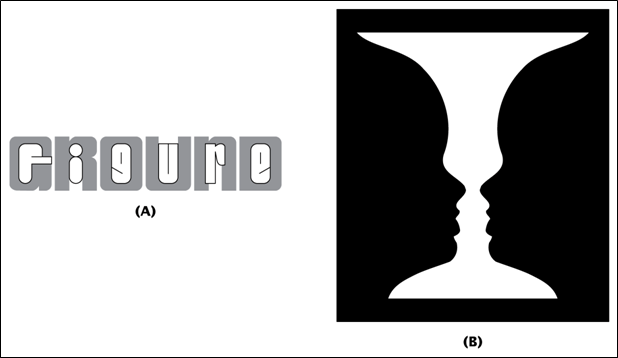
\includegraphics[width=0.5\textwidth]{FIGURES/figground1}\\
    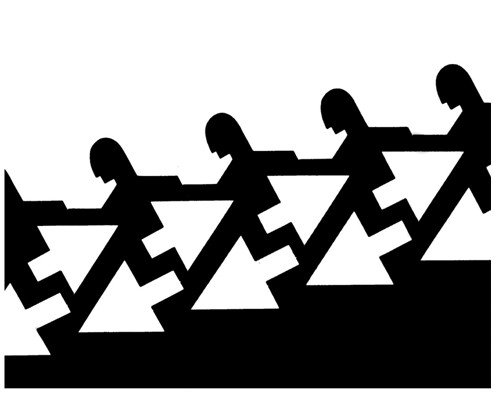
\includegraphics[width=0.5\textwidth]{FIGURES/figground2}\\
  \end{center}
  \vfill
  {\fontsize{6}{6}\selectfont Slide adapted from ``Sensation and Perception'' at \texttt{http://college.cengage.com}}
\end{frame}


\begin{frame}[t]{Grouping}
  \begin{center}
    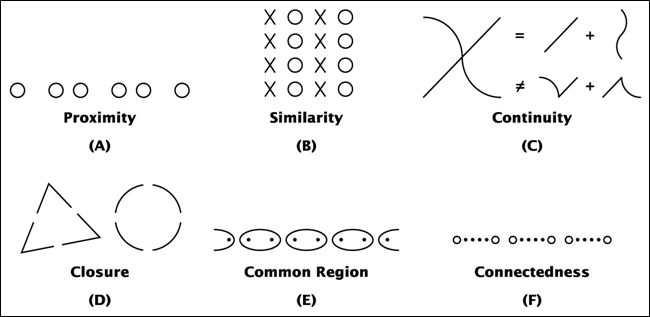
\includegraphics[width=0.5\textwidth]{FIGURES/perceptgrouping1}\\
    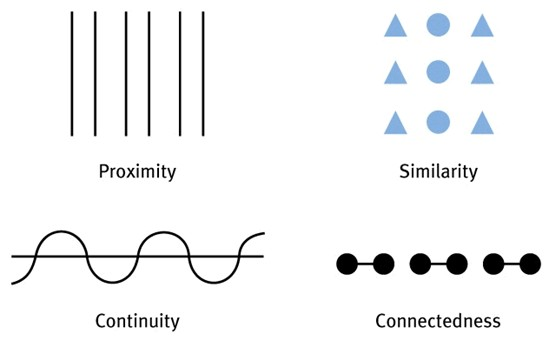
\includegraphics[width=0.5\textwidth]{FIGURES/perceptgrouping2}\\
  \end{center}
  \vfill
  {\fontsize{6}{6}\selectfont Slide adapted from ``Sensation and Perception'' at \texttt{http://college.cengage.com}}
\end{frame}

\begin{frame}[t]{Operationalization}
  \begin{itemize}
  \item Similarity and Common Regions principles. Detect coherent regions, a.k.a \myemph{segments}. Group them further.
    \begin{center}
      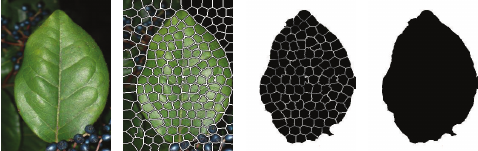
\includegraphics[width=0.8\textwidth]{FIGURES/SegGrouping}
    \end{center}
  \item Two different segments should have dissimilar properties. In
    particular, boundary between segments should present large
    variations.\vfill
  \item Two main approaches: \vfill
    \begin{itemize}
    \item Region based segmentation. \vfill
    \item Edge / contour based segmentations.\vfill
    \end{itemize}
  \end{itemize}
\end{frame}



%-----------------------------------------------------------

\begin{frame}
  \frametitle{Regions and Edges}
  \begin{itemize}
  \item A region should be bounded by a closed contour: edge
    detection.
  \item Regions may be obtained by ``boundary filling''.\vfill
  \item However edges are not always well defined in observed images. 
  \end{itemize}
  \pause
  \begin{center}
    \visible<2->{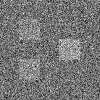
\includegraphics[width=0.25\textwidth]{IMAGES/noisy_squares}}
  \end{center}
\end{frame}


%----------------------------------------------------------


\begin{frame}
  \frametitle{Regions}
  \begin{itemize}
  \item Regions correspond generally to objects or pieces of objects in a scene. 
  \item Scenes may contain several objects.
  \end{itemize}
  \begin{center}
    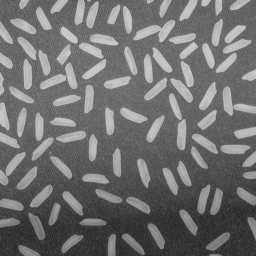
\includegraphics[width=0.4\textwidth]{IMAGES/rice}
 \end{center}
\end{frame}



%-----------------------------------------------------------
\section{Edge recovery}


\begin{frame}
  \frametitle{Edge Based Segmentation}
  \begin{itemize}
  \item Boundary between region corresponds to sharp intensity / color / texture change.
  \item Derivatives should indicate this:
    \begin{center}
      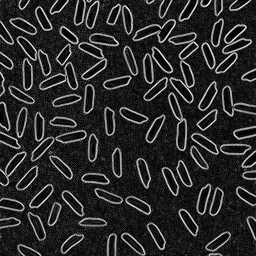
\includegraphics[width=0.25\textwidth]{IMAGES/ricegradient}
    \end{center}
  \item Edges should correspond to local maximum of gradient magnitude.
  \item Gradient of $f$ : $\nabla f = (f_x,f_y)^T$, Gradient magnitude = $\sqrt{f_x^2 + f_y^2}$.
  \item Zero-crossing of Laplacian $\Delta f = \nabla^2 f := f_{xx} + f_{yy}$ is also an indicator.
  \item How to compute image derivatives / gradient?
  \end{itemize} 
  
\end{frame}


%---------------------------------------------------------------
\begin{frame}
  \frametitle{Image Derivatives - First Order}
  \begin{itemize}
  \item Finite difference approximation:
    \begin{itemize}{\fontsize{8}{6}\selectfont
    \item  Forward differences
      $$
      \pder{f(x,y)}{x} \approx \frac{f(x+h,y)-f(x,y)}{h},\quad \pder{f(x,y)}{y} \approx \frac{f(x,y+h)-f(x,y)}{h}
      $$ 
    \item Backward differences
      $$
      \pder{f(x,y)}{x} \approx \frac{f(x,y)-f(x-h,y)}{h},\quad \pder{f(x,y)}{y} \approx \frac{f(x,y)-f(x,y-h)}{h}
      $$ 
    \item Central differences
      $$
      \pder{f(x,y)}{x} \approx \frac{f(x+h,y)-f(x\!-\!h,y)}{2h}, \pder{f(x,y)}{y} \approx \frac{f(x,y+h)\!-\!f(x,y\!-\!h)}{2h}
      $$ 
    }
    \end{itemize}
  \item For those familiar with it, they can be implemented by convolution!
  \end{itemize}
\end{frame}

\begin{frame}
  \frametitle{Second Order Derivatives}

  \begin{itemize}{\fontsize{8}{6}\selectfont
  \item $xx$-direction
    $$
    \pderd{2}{f(x,y)}{x^2} \approx\frac{f(x+h,y)-2f(x,y)+f(x-h,y)}{h^2},
    $$
  \item $yy$-direction
    $$
    \pderd{2}{f(x,y)}{y^2} \approx\frac{f(x,y+h)-2f(x,y)+f(x,y-h)}{h^2},
    $$
  \item $xy$-direction
    \begin{align*}
    \pderd{2}{f(x,y)}{x\partial y}\approx \frac{1}{4h^2}&\Big(
      -f(x-h,y+h) +f(x+h,y+h)\\
      &+f(x-h,y-h)  -f(x+h,y-h)\Big)
    \end{align*}
  \item Here too, convolution!
  }
  \end{itemize}
\end{frame}




\begin{frame}
  \frametitle{Derivatives and noise}
  \begin{itemize}
  \item Derivation filters are high pass: they amplify high pass signals and noise is high pass.
  \item Solution: Apply smoothing filter prior to differentiation.\vfill 
  \item Better: combine smoothing filter and differentiation!\vfill
  \item Remember S{\o}ren's lectures!
    $$
    D\left( g\ast f\right) = Dg\ast f
    $$
  \end{itemize}
\end{frame}


\begin{frame}
  \frametitle{Derivatives and Gaussian, Again S{\o}ren's lectures}
  \begin{itemize} 
  \item Convolution by Gaussian smooths: noise removal. Standard
    deviation of Gaussian directly linked to \myemph{scale} of
    features.
  \item Derivative of Gaussian:
    $$
    g_\sigma = \frac{1}{2\pi\sigma^2}e^{-\frac{x^2 + y^2}{2\sigma^2}},\quad \pder{g_\sigma}{x} = -\frac{x}{\sigma^2}g_\sigma,\quad
    \pder{g_\sigma}{y} = -\frac{y}{\sigma^2}g_\sigma
    $$
  \item Laplacian of Gaussian (LoG)
    $$
    \Delta g_\sigma = \pderd{2}{g_\sigma}{x^2} +  \pderd{2}{g_\sigma}{y^2} = \frac{x^2 + y^2 - 2\sigma^2}{\sigma^4}g_\sigma
    $$
  \end{itemize}
\end{frame}



%----------------------------------------------------------

\begin{frame}
  \frametitle{Marr-Hildreth Edge Detector}
  D. Marr and E. Hildreth, 1980.
  \begin{itemize}
  \item Observe zero-crossing of Laplacian of Gaussian (the same use for SIFT for instance)
  \item Convolve image $f$ with Laplacian of Gaussian filter: $\Delta_\sigma f = \Delta g_\sigma \ast f$  
  \item Detect the zero-crossings of $\Delta_\sigma f$
  \end{itemize}
  \begin{center}
    \begin{tabular}[h]{cc}
      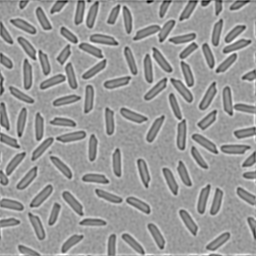
\includegraphics[width = 0.2\textwidth]{IMAGES/lorice1_4}& 
      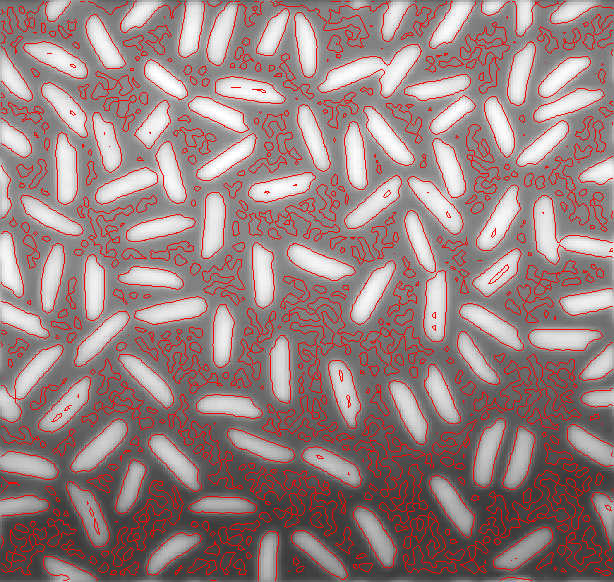
\includegraphics[width = 0.21\textwidth]{IMAGES/riceedges1_4mh}\\
      LoG $\sigma = 1.4$ & detected edges
    \end{tabular}\\
    \begin{tabular}[h]{cc}
      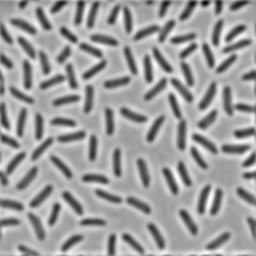
\includegraphics[width = 0.2\textwidth]{IMAGES/lorice3_0}& 
      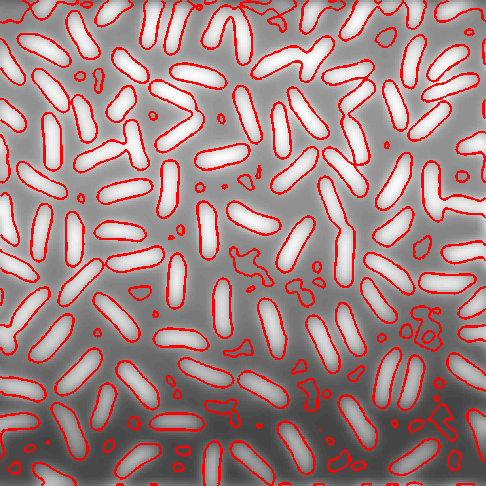
\includegraphics[width = 0.2\textwidth, height = 0.2\textwidth]{IMAGES/riceedges3_0mh}\\
      LoG $\sigma = 3.0$ & detected edges
    \end{tabular}\\
  \end{center}
\end{frame}



%--------------------------------------------------------------


\begin{frame}
  \frametitle{Canny Edge Detector}
  J. Canny, 1986.
  \begin{itemize}
  \item Develop an algorithm optimal wrt:
    \begin{itemize}
    \item Detection: maximize probability of detection of true edges, minimize probability of detection of false ones.\vfill
    \item Localization: detected edges as close as possible to real ones.\vfill
    \item Number of responses: 1 real edge should not result in 2 or
      more detected ones.\vfill
    \end{itemize}
  \item Canny algorithm attempts to answer optimally to these criteria.
  \item Divided in 5 steps.
  \end{itemize}
\end{frame}


\begin{frame}
  \frametitle{Algorithm - I}
  \begin{enumerate}
  \item \myemph{Smoothing}. Noise removal by Gaussian smoothing with 2D-Gaussian $g_\sigma$.
  \item \myemph{Gradient computation}. Can be combined with step 1 by
    convolution with Gaussian derivatives. Gives $f_{x\sigma}$ and
    $f_{y\sigma}$. Potential edges marked as gradients with large
    magnitudes. Directions computed by
    $$
    \theta = \arctan\left(\frac{|f_{y\sigma}|}{|f_{x\sigma}|}\right).
    $$
  \item \myemph{Non-maximum suppression.} 
    \begin{itemize}
    \item Round gradient direction to nearest $45^\circ$ (connectivity of a 8-points neighborhood).
    \item Compare gradient magnitude of current pixel with magnitudes
      of neighbors in the gradient direction. That is, if $\theta =
      90^\circ$ compare with north and south pixel, if $\theta =
      135^\circ$ compare with ? (\myemph{this is a question for you!}) 
    \item If gradient magnitude of the current pixel is largest, keep
      it, otherwise suppress it (say set to 0).
    \end{itemize}
  \end{enumerate}
\end{frame}


\begin{frame}
  \frametitle{Algorithm - II}
  \begin{enumerate}
  \item \myemph{Double thresholding}. Non suppressed edges marked with their gradient magnitude. Some are true edges, some may be noise.
    Two thresholds $\tau_{high}$ and $\tau_{low}$ are used. Edges with magnitude $\geq \tau_{high}$ marked as \myemph{strong edges}.
     Edges with magnitude between$\tau_{low}$ and $\tau_{high}$ marked as \myemph{weak edges}. Remaining are suppressed.\vfill
   \item \myemph{Hysteresis edge tracking} Strong edges are certain
     and included in the final image.  Weak edges included only if
     connected (via other weak edges) to strong edges. Connectivity
     means existence of a chain of neighbor weak edges pixels from
     candidate edge to a strong edge.
  \end{enumerate}
\end{frame}

%-----------------------------------------------------------

\begin{frame}
  \frametitle{Canny Example}
  $\tau_{low} = 0.08$, $\tau_{high} = 0.2$
  \begin{center}
    \begin{tabular}[h]{ccc}
      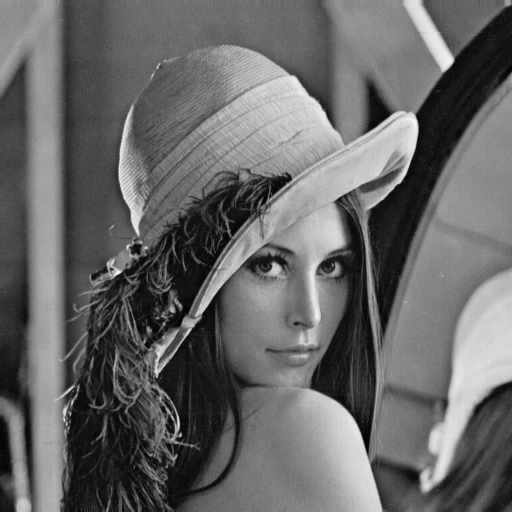
\includegraphics[width=0.3\textwidth]{IMAGES/lena} &
      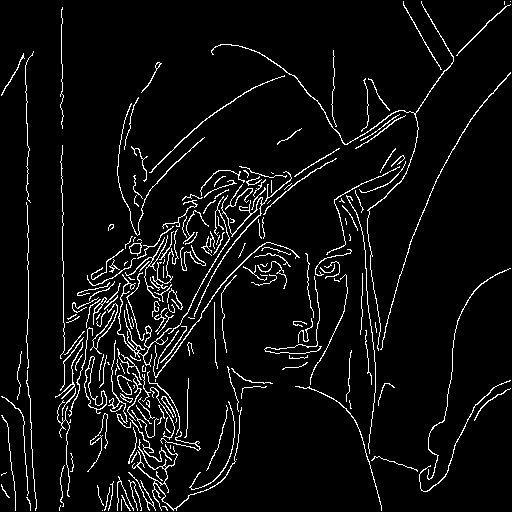
\includegraphics[width=0.3\textwidth]{IMAGES/edgelena1_4_0_2} &
      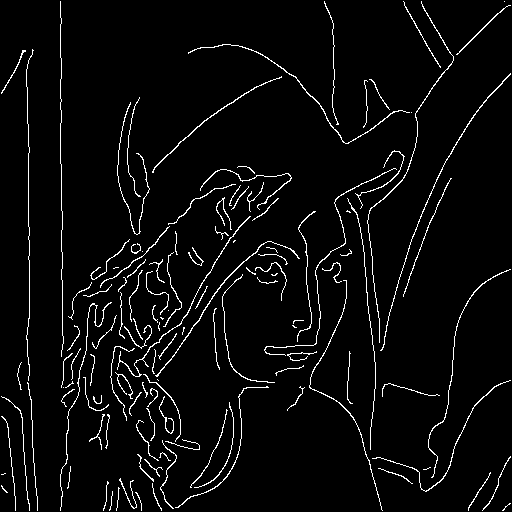
\includegraphics[width=0.3\textwidth]{IMAGES/edgelena3_0_0_2} \\
      source image & $\sigma=1.4$ & $\sigma=3.0$
    \end{tabular}
  \end{center}
  \begin{itemize}

  \item Edges are not closed: good but might be insufficient for segmentation.
  \end{itemize}
\end{frame}


%-------------------------------------------------------------------

\section{Closing the gaps: Active Contours}


\begin{frame}
  \frametitle{Contours and Perception: Amodal Completion }
   A Classical example from Italian psychologist G. Kanizsa\footnote{Grammatica del vedere / Organization in Vision}
   \begin{center}
     \begin{tabular}[h]{cc}
        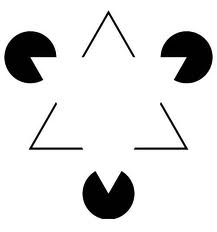
\includegraphics[width=0.3\textwidth]{IMAGES/kanizsa1} &
      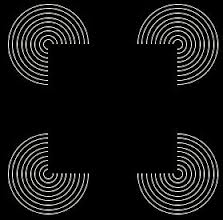
\includegraphics[width=0.3\textwidth]{IMAGES/kanizsa2} \\
     \end{tabular}
   \end{center}
   The brain is ``closing the gaps'' -- Gestalt's closure principle.
\end{frame}

\begin{frame}
  \frametitle{But how...}
  What is the best continuation?
   \begin{center}
     \begin{tabular}[h]{cc}
        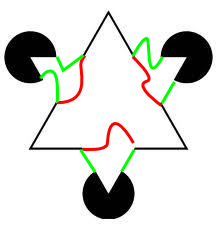
\includegraphics[width=0.3\textwidth]{IMAGES/kanizsa1bad} &
      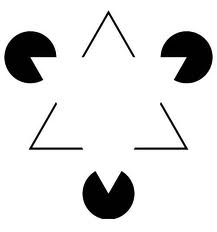
\includegraphics[width=0.3\textwidth]{IMAGES/kanizsa1ok} \\
     \end{tabular}
   \end{center}
   \begin{itemize}
   \item  We reconstruct the gap with an implicit assumption of simplicity / regularity for the contour.
   \item  Variational segmentation algorithms operationalize it.
   \end{itemize}

\end{frame}



\begin{frame}
  \frametitle{Contour representation}
  \begin{itemize}
  \item The simplest way to represent a 2D contour is to use a curve.
  \item Mathematically, it is a function
    $$
    C: p\in[a,b] \mapsto C(p) = (x(p), y(p))\in \RR^2
    $$
  \item If $C(a) = C(b)$ the curve is closed.
  \end{itemize}
  \begin{columns}
    \column{0.5\textwidth}
    \vspace{-5mm}
    \begin{center}
       $t\mapsto(\cos(p),\sin(p)$\\
    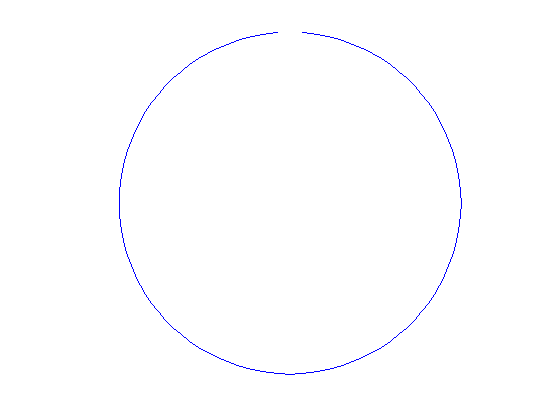
\includegraphics[width=0.8\textwidth]{FIGURES/simplecircle}
    \end{center}
   \column{0.5\textwidth}
    $p\mapsto(\cos(2p)^2,\sin(p)\cos(3p)$
    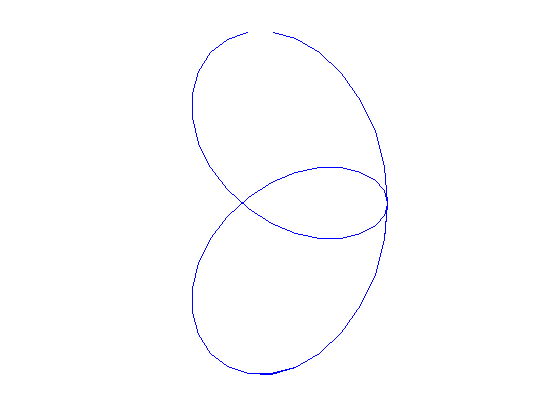
\includegraphics[width=0.8\textwidth]{FIGURES/butterfly}
  \end{columns}
\end{frame}


\begin{frame}
  \frametitle{Simplicity / Regularity}
  \begin{center}
    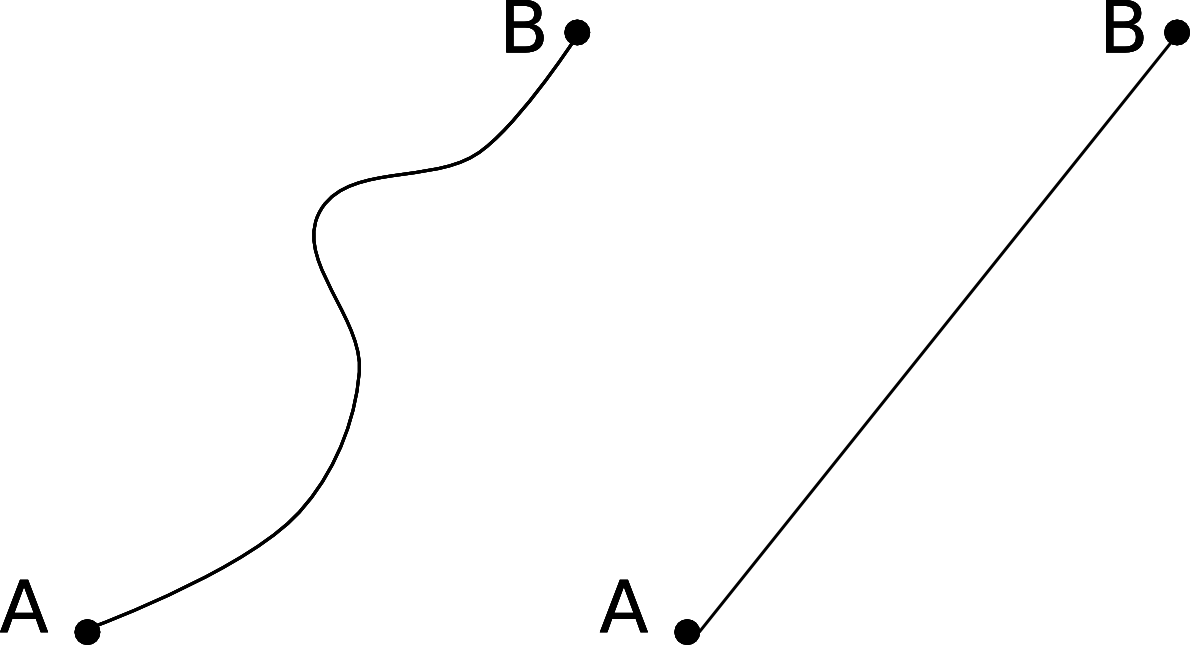
\includegraphics[width=0.6\textwidth]{FIGURES/curvessimplecomplex}
  \end{center}
  \begin{itemize}
  \item The first curve is longer and winds more than the second one.
  \item The second one is simpler.
  \end{itemize}
\end{frame}

\begin{frame}\frametitle {Snakes, Kass, Witkin, Terzopoulos 1988}
  \begin{itemize}
  \item Curves evolving (as snakes) to catch an object. Also called Active Contours.
  \item How to define the``Cost of a Segmentation'':
  \item \myemph{Cost} of a curve lying on an image such that
    \begin{itemize}
    \item The more a curve follows edges of the image, the ``cheaper'' it is. \vfill
    \item The more a curve is bending / winding, the ``more expensive'' it is.\vfill
    \item Design an algorithm to compute the ``minimal cost'', or a cost low enough. \vfill
    \item Kass, Witkin. Terzopoulos: minimize
      $$
      \Ee(C) = \int \alpha|\dot{C}|^2+ \beta|\ddot{C}|^2\,dt + \int F_{\text{edge}}(C(t))\,dt
      $$
    \item Solution via Partial Differential Equation (PDE).\vfill
    \item  Start with initial contour. Evolve it so as to decrease cost as fast as possible (steepest descent).\vfill
    \item Thousands of derived methods!
    \end{itemize}
  \end{itemize}

\end{frame}




\begin{frame}[t]{Active Contour Example}
  \begin{center}
    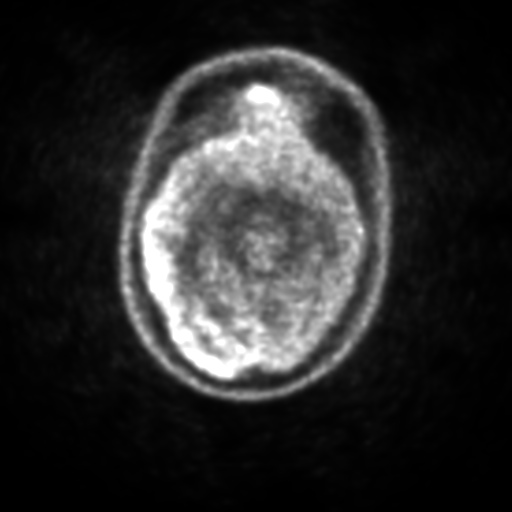
\includegraphics[width=0.2\textwidth]{FIGURES/PET}
  \end{center}
  \begin{center}
    \begin{tabular}[h]{ccc}
       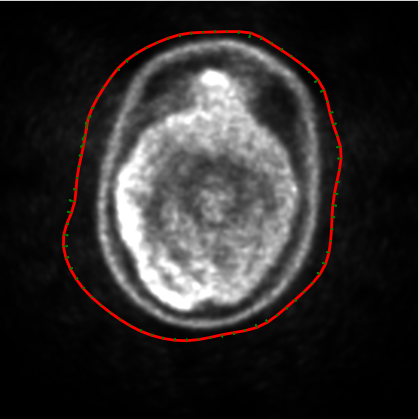
\includegraphics[width=0.2\textwidth]{FIGURES/PET1}&
       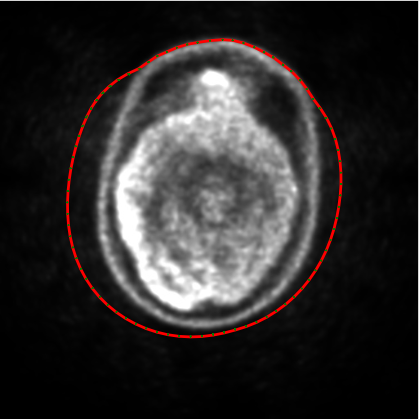
\includegraphics[width=0.2\textwidth]{FIGURES/PET2}&
       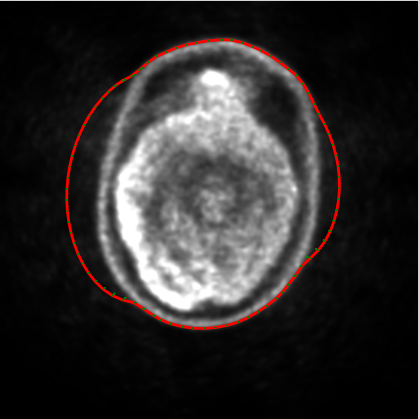
\includegraphics[width=0.2\textwidth]{FIGURES/PET3}\\
       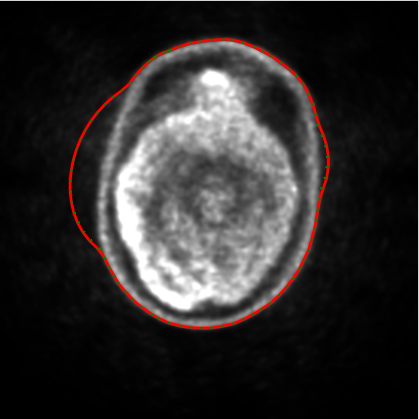
\includegraphics[width=0.2\textwidth]{FIGURES/PET4}&
       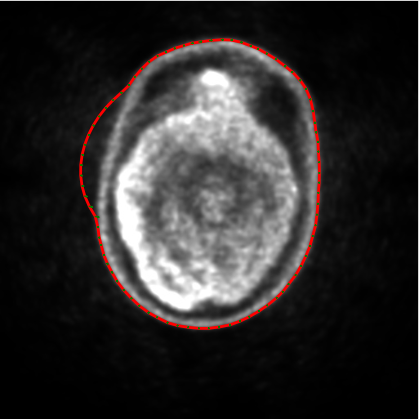
\includegraphics[width=0.2\textwidth]{FIGURES/PET5}&
       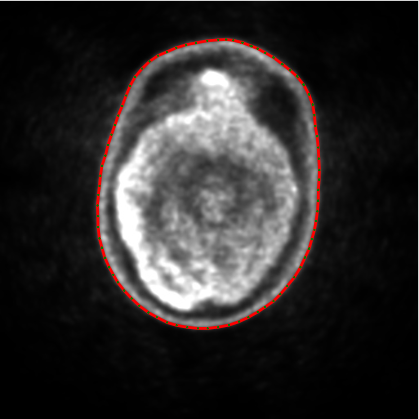
\includegraphics[width=0.2\textwidth]{FIGURES/PET6}
    \end{tabular}
  \end{center}
\end{frame}

\section{Content Similarity: Clustering Methods}
\label{sec:clus}

\begin{frame}[t]{Clusters of Features}

  \begin{itemize}
  \item Idea: extract features for each pixel of the image.\vfill
  \item Group features by similarity.\vfill
  \item Regions with similar features = segments.\vfill
  \item Need to define what features are.\vfill
  \item Need to define what feature similarity is.\vfill
  \item Automatic determination of clusters? Choice of the number of clusters?
  \end{itemize}
\end{frame}


\begin{frame}[t]{Clustering In General}
  \begin{center}
    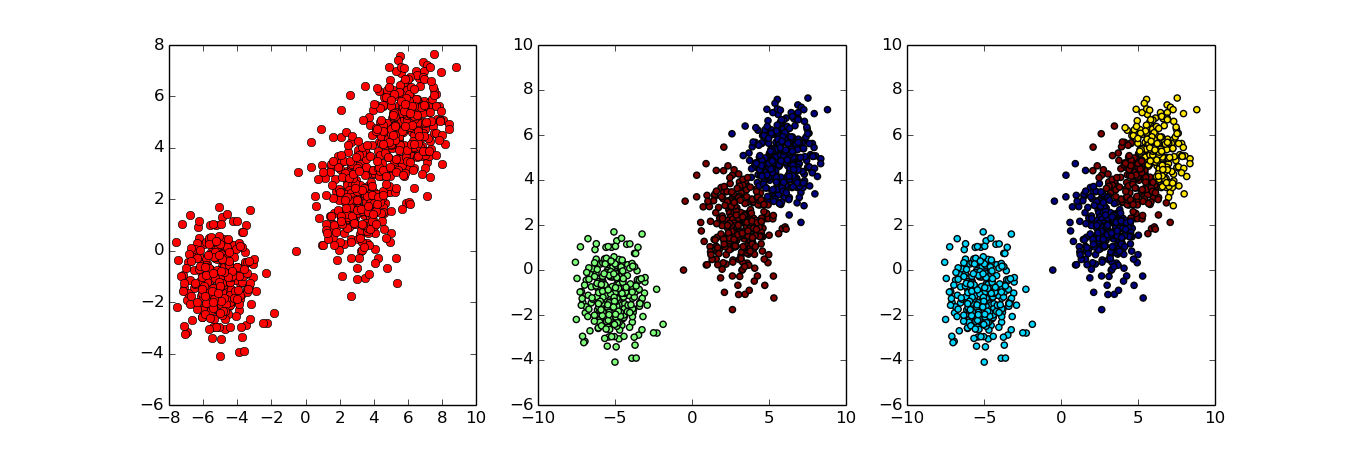
\includegraphics[width=0.8\textwidth]{FIGURES/kmeans34classes}\\
    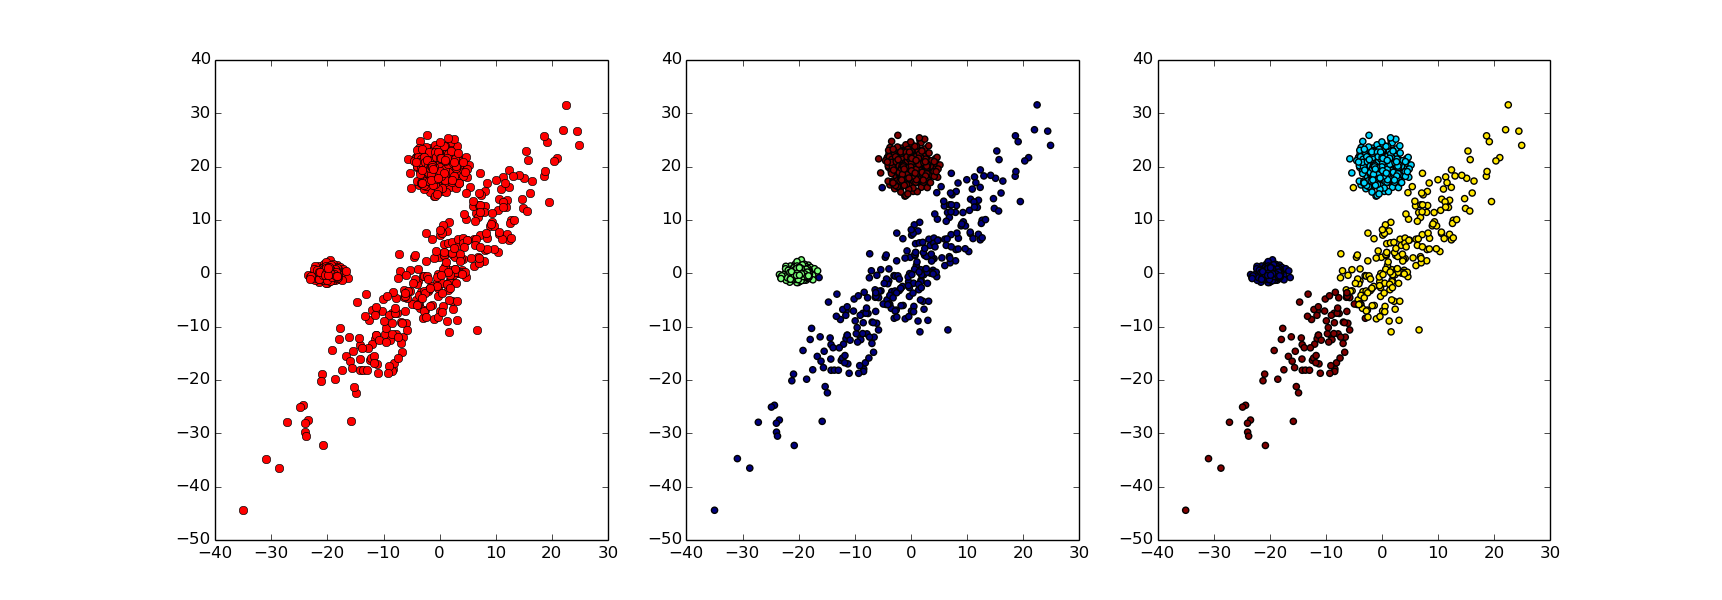
\includegraphics[width=0.8\textwidth]{FIGURES/GMM34classes}\\
  \end{center}
  ~\\
  Up: $k$-means clustering, with $k$ = 3, 4. (3 = optimal)
  Down: Gaussian Mixture models with $3$ and  $4$ ($3$ optimal too).
\end{frame}


\begin{frame}[t]{The $k$-Means Algorithm}
  \begin{columns}
    \begin{column}{0.4\textwidth}
      \begin{center}
        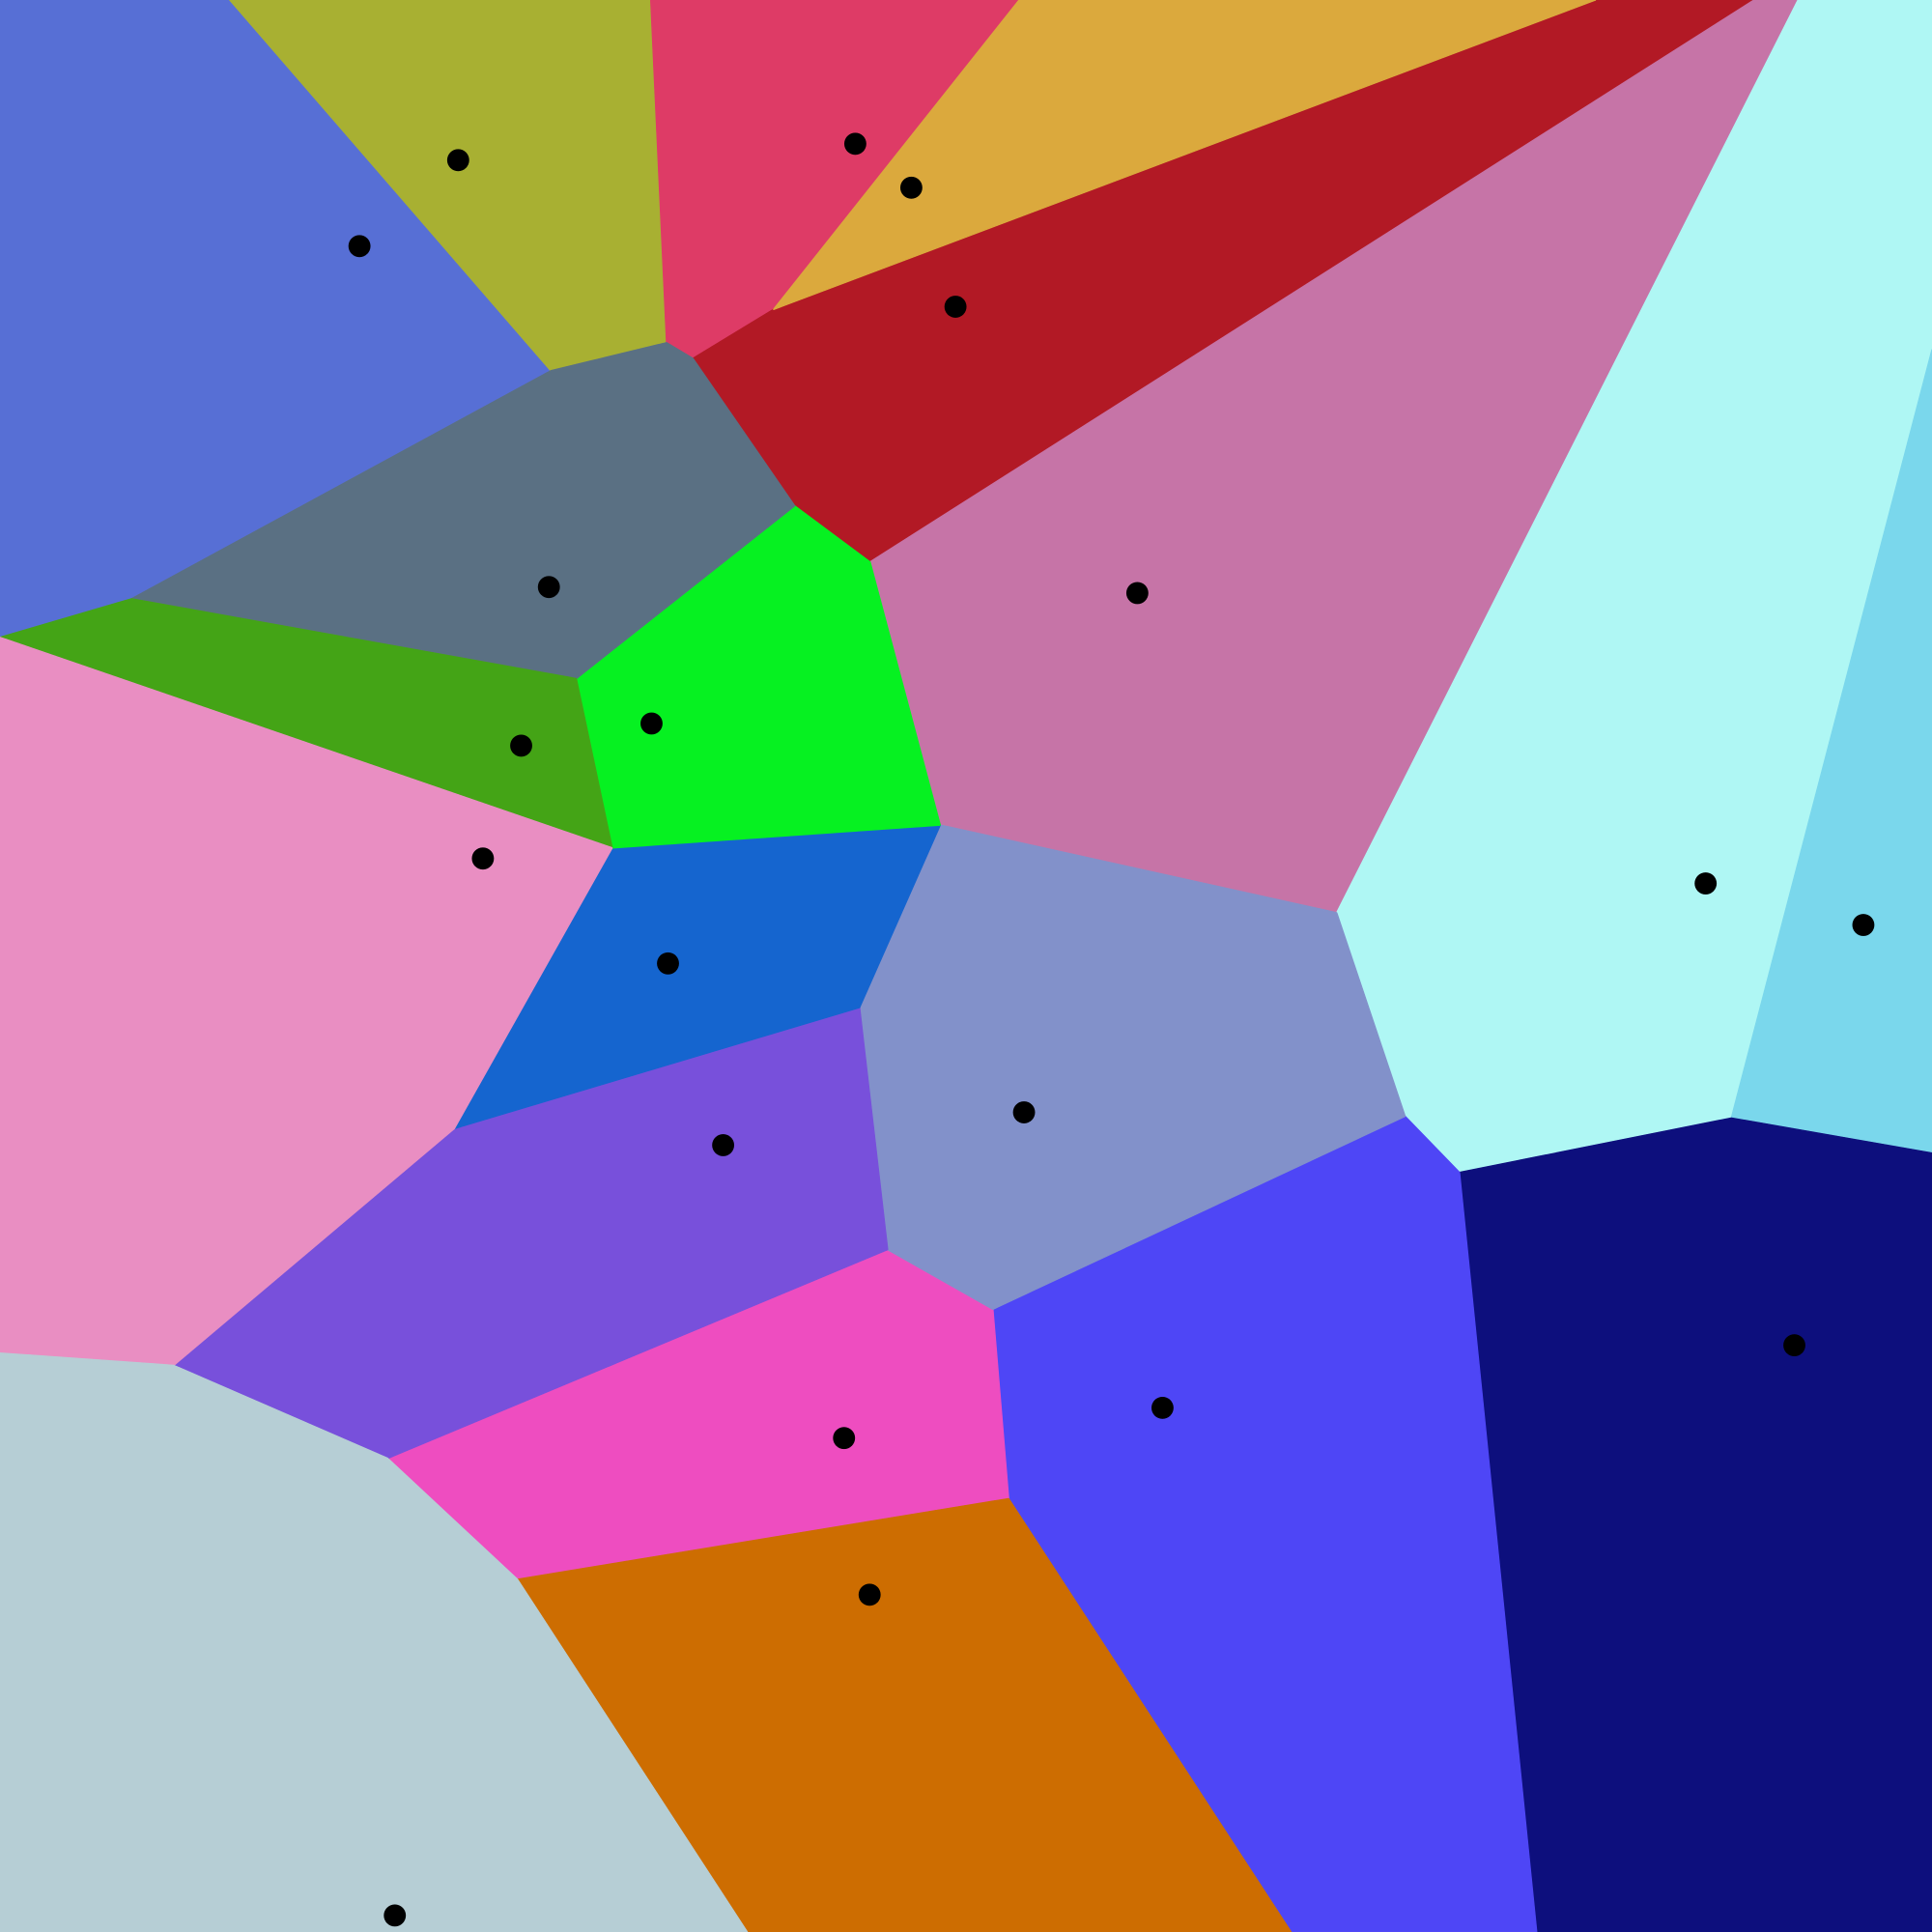
\includegraphics[width=0.8\textwidth]{FIGURES/Euclidean_Voronoi_diagram}
      \end{center}
    \end{column}
    \begin{column}{0.6\textwidth}
      \begin{itemize}
      \item Plan divided into cells.
      \item Proximity to centroid.
      \item $k$-means: compute centroids, implicit Vorono{\"i} tessellation, from data.
      \item Remember S{\o}ren's lecture from Monday!
      \end{itemize}
    \end{column}
  \end{columns}
  \begin{itemize}
  \item $X = \{x_1,\dots,x_n\}$ set of data points. Find a partition $S_1,\dots,S_k$ of $X$ and points $\mu_1,\dots,\mu_k$ such that
    $$
    \Dd(S_1\dots,S_k) = \sum_{j=1}^k\sum_{x\in S_j}\|x-\mu_j\|^2 = \text{ minimum}.
    $$
  \item The $\mu_j$s are the centroids of the $S_j$s.
  \end{itemize}
\end{frame}



\begin{frame}[t]{Lloyd's Algorithm}
  \begin{itemize}
  \item Start with $k$ candidate centroids. How to choose them?
  \item Repeat:
    \begin{enumerate}
    \item Label pixels / assign them to clusters from their feature distance to centroids.
    \item Recompute centroids of features as average of clusters
    \end{enumerate}
  \item until regions or centroids don't change.
  \end{itemize}
  ~\\
  \begin{itemize}
  \item What are good features for segmentation?
  \item Depends on image content.
  \end{itemize}
\end{frame}


\begin{frame}[t]{Gaussian Scale Space Features}
  \begin{itemize}
  \item 4 scales, $\sigma = 0.5, 1.0, 2.0, 4.0$
  \item Gaussian derivatives from order 0 (no derivative) to order 3
    $$
    \pderd{0}{}{x^0\partial
      y^0},\pder{}{x},\pder{}{y},\pderd{2}{}{x^2},\pderd{2}{}{y^2},\pderd{2}{}{x\partial
      y},\pderd{3}{}{x^3},\pderd{3}{}{y^3},\pderd{3}{}{x^2\partial
      y},\pderd{3}{}{x\partial y^2}
    $$
  \item In all, 40 features per pixel!
  \end{itemize}
  
  \begin{center}
    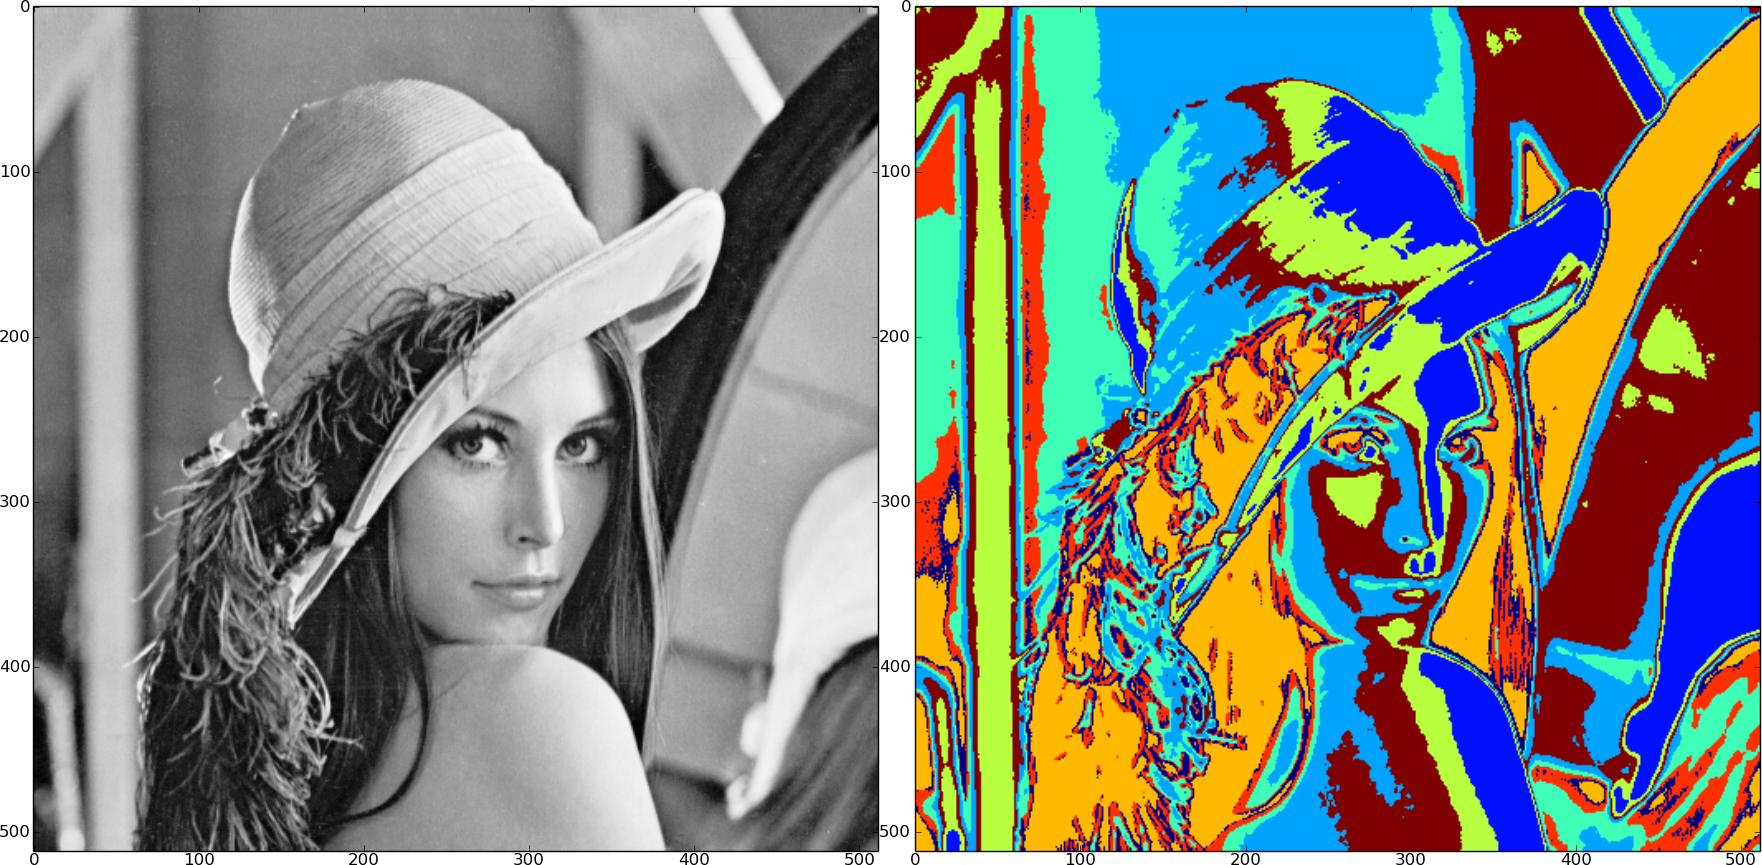
\includegraphics[width=0.6\textwidth]{FIGURES/Seg_lena_8_order2_4scales_with_intensity}
  \end{center}
 
  
\end{frame}


\begin{frame}[t]{Variation}
  \begin{itemize}
  \item Same features, but without order 0 (intensity)
  \end{itemize}
  \begin{center}
    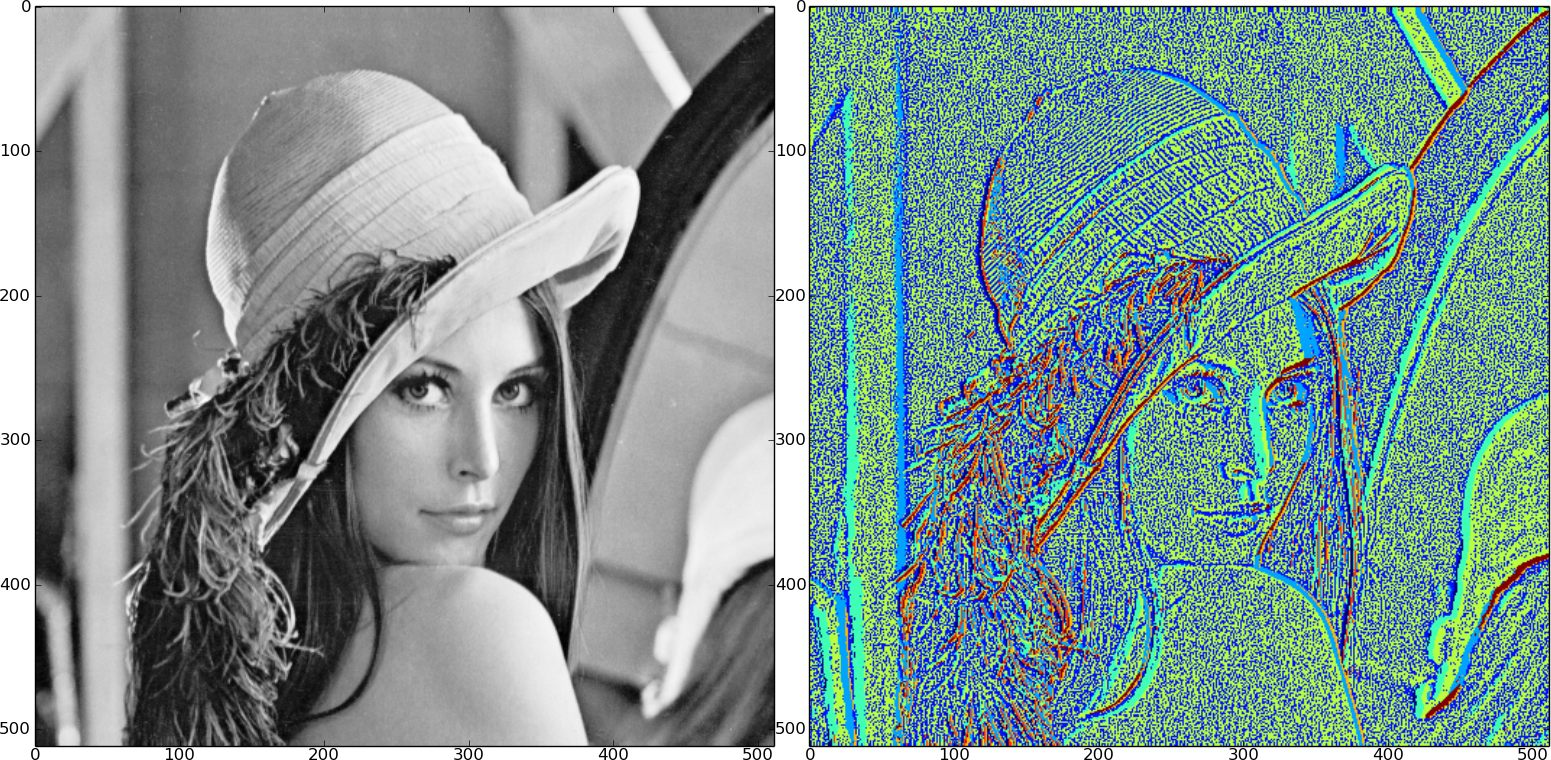
\includegraphics[width=0.6\textwidth]{FIGURES/Seg_lena_8_order2_4scales_no_intensity}
  \end{center}
  \begin{itemize}
  \item Conclusion: a lot of information in intensity alone!
  \end{itemize}
  \pause
  \begin{center}
    \visible<2->{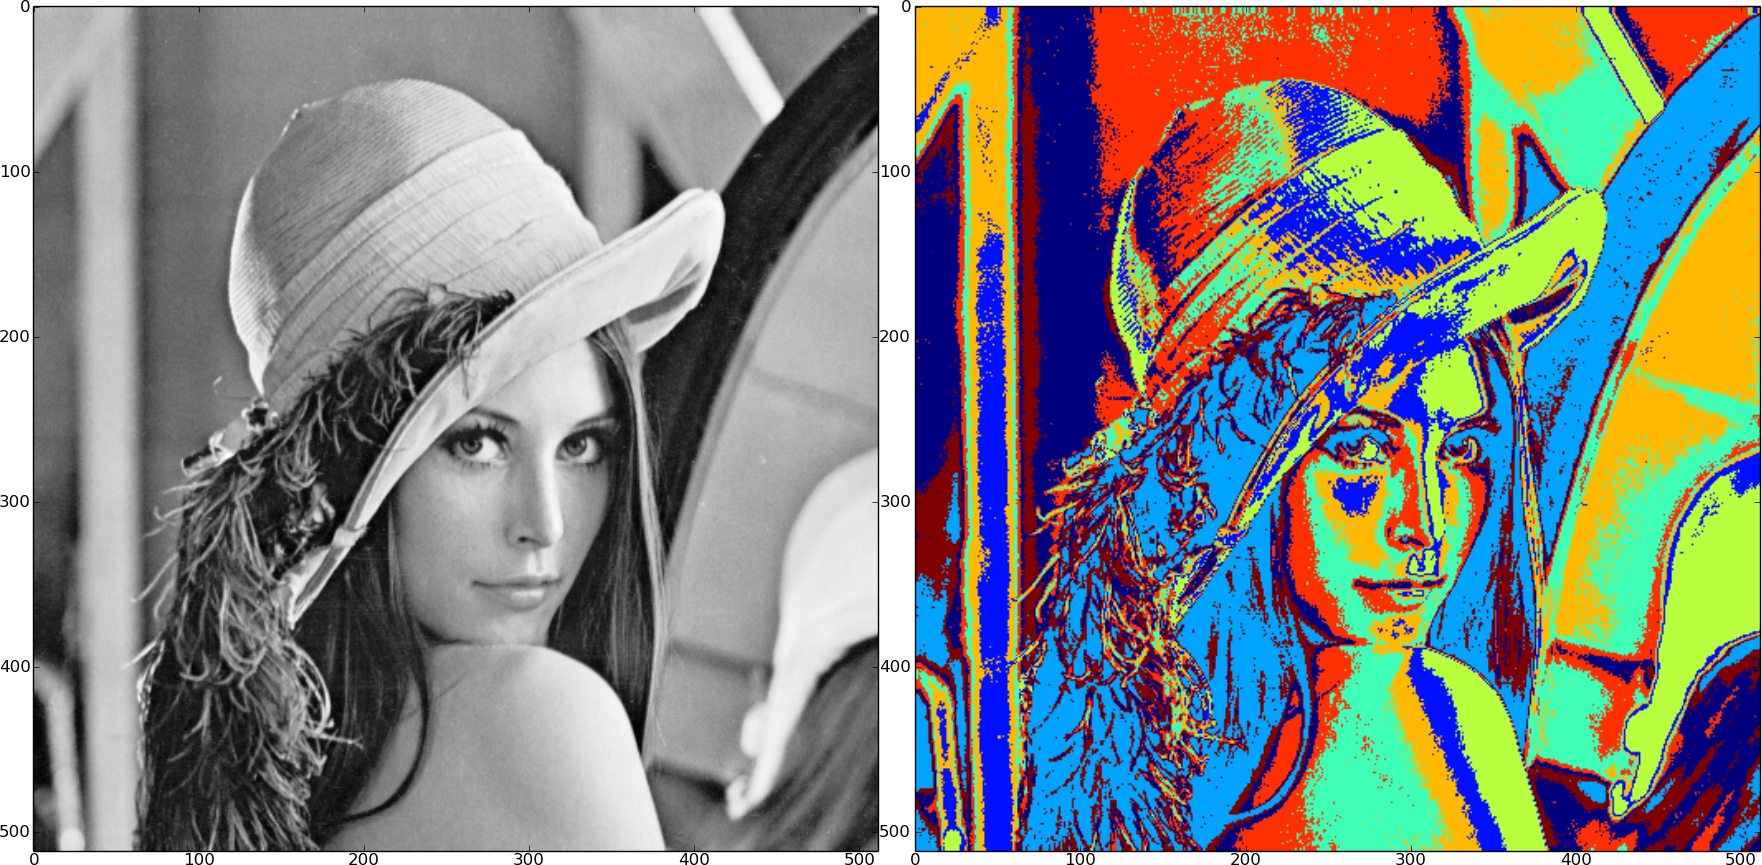
\includegraphics[width=0.6\textwidth]{FIGURES/Seg_lena_8_noscaley}}
  \end{center}

\end{frame}


\begin{frame}[t]{Choice of $k$}
  \begin{itemize}
    \item Previous image clearly over segmented.
  \item (smoothed) histogram of Lena Image $\pm$ 8 ``bumps'':
    \begin{center}
      \only<1>{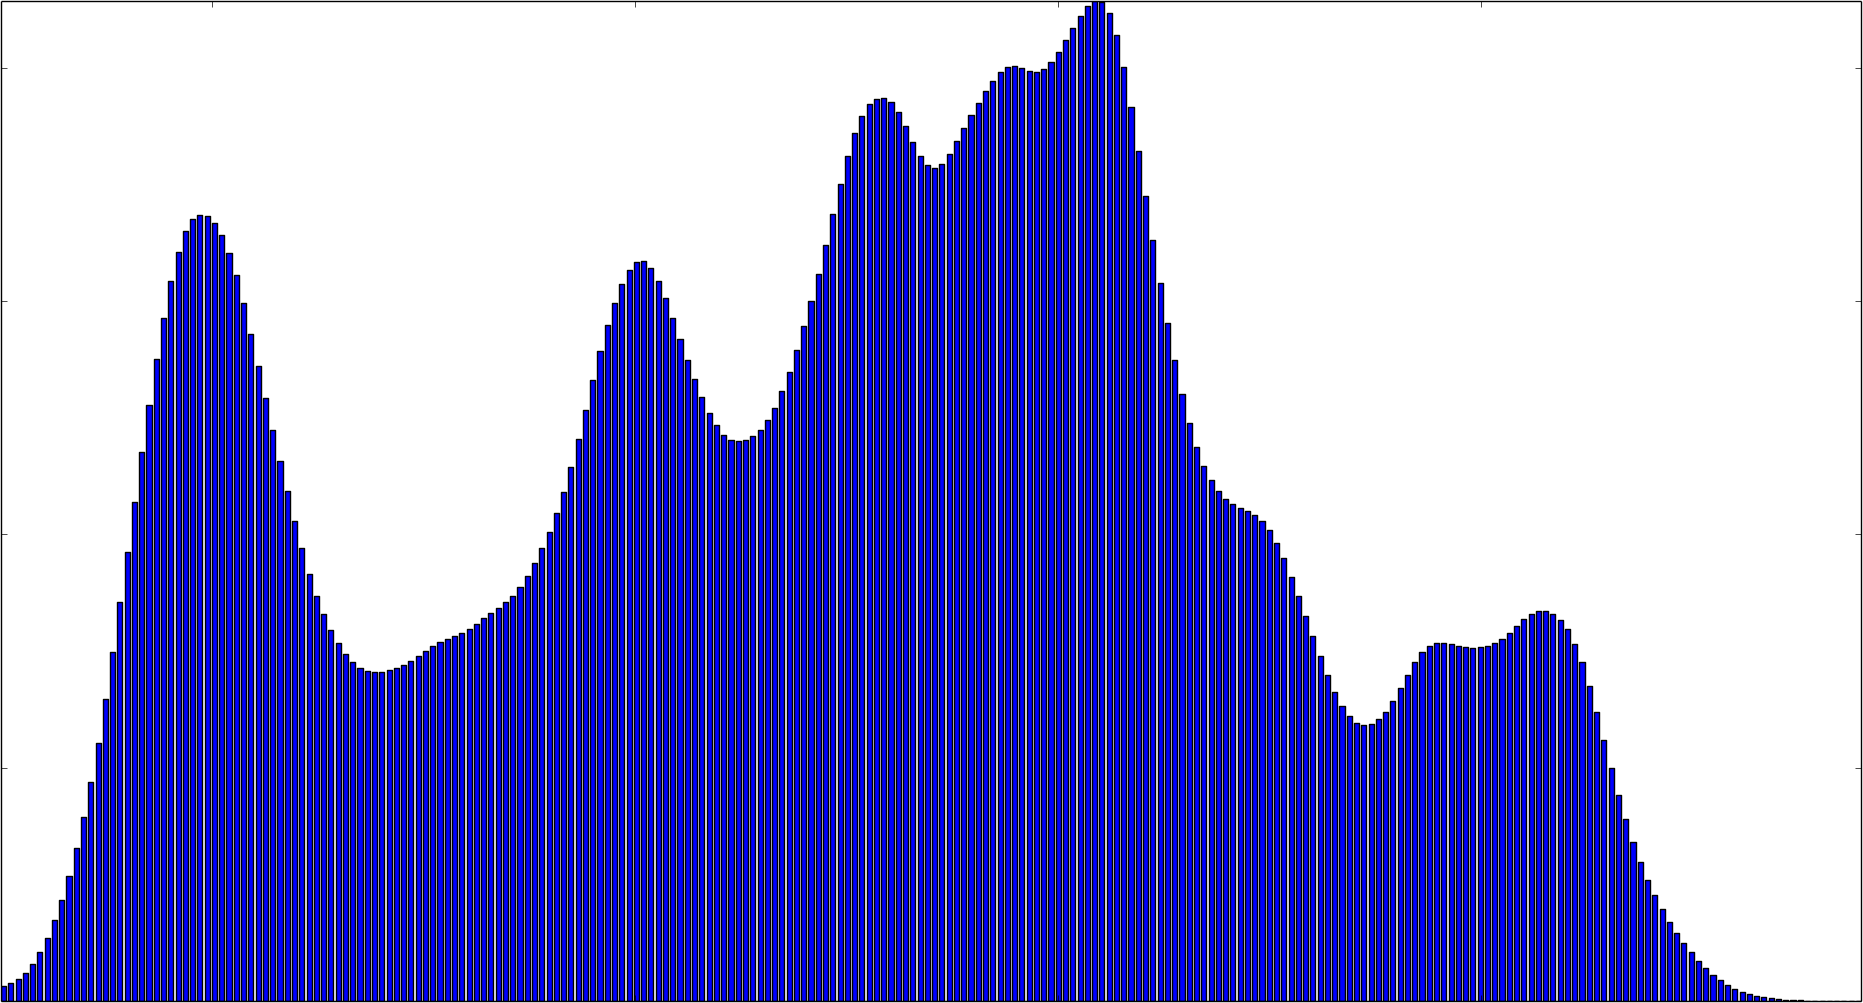
\includegraphics[width=0.7\textwidth]{FIGURES/lena_histogram}}
      \only<2->{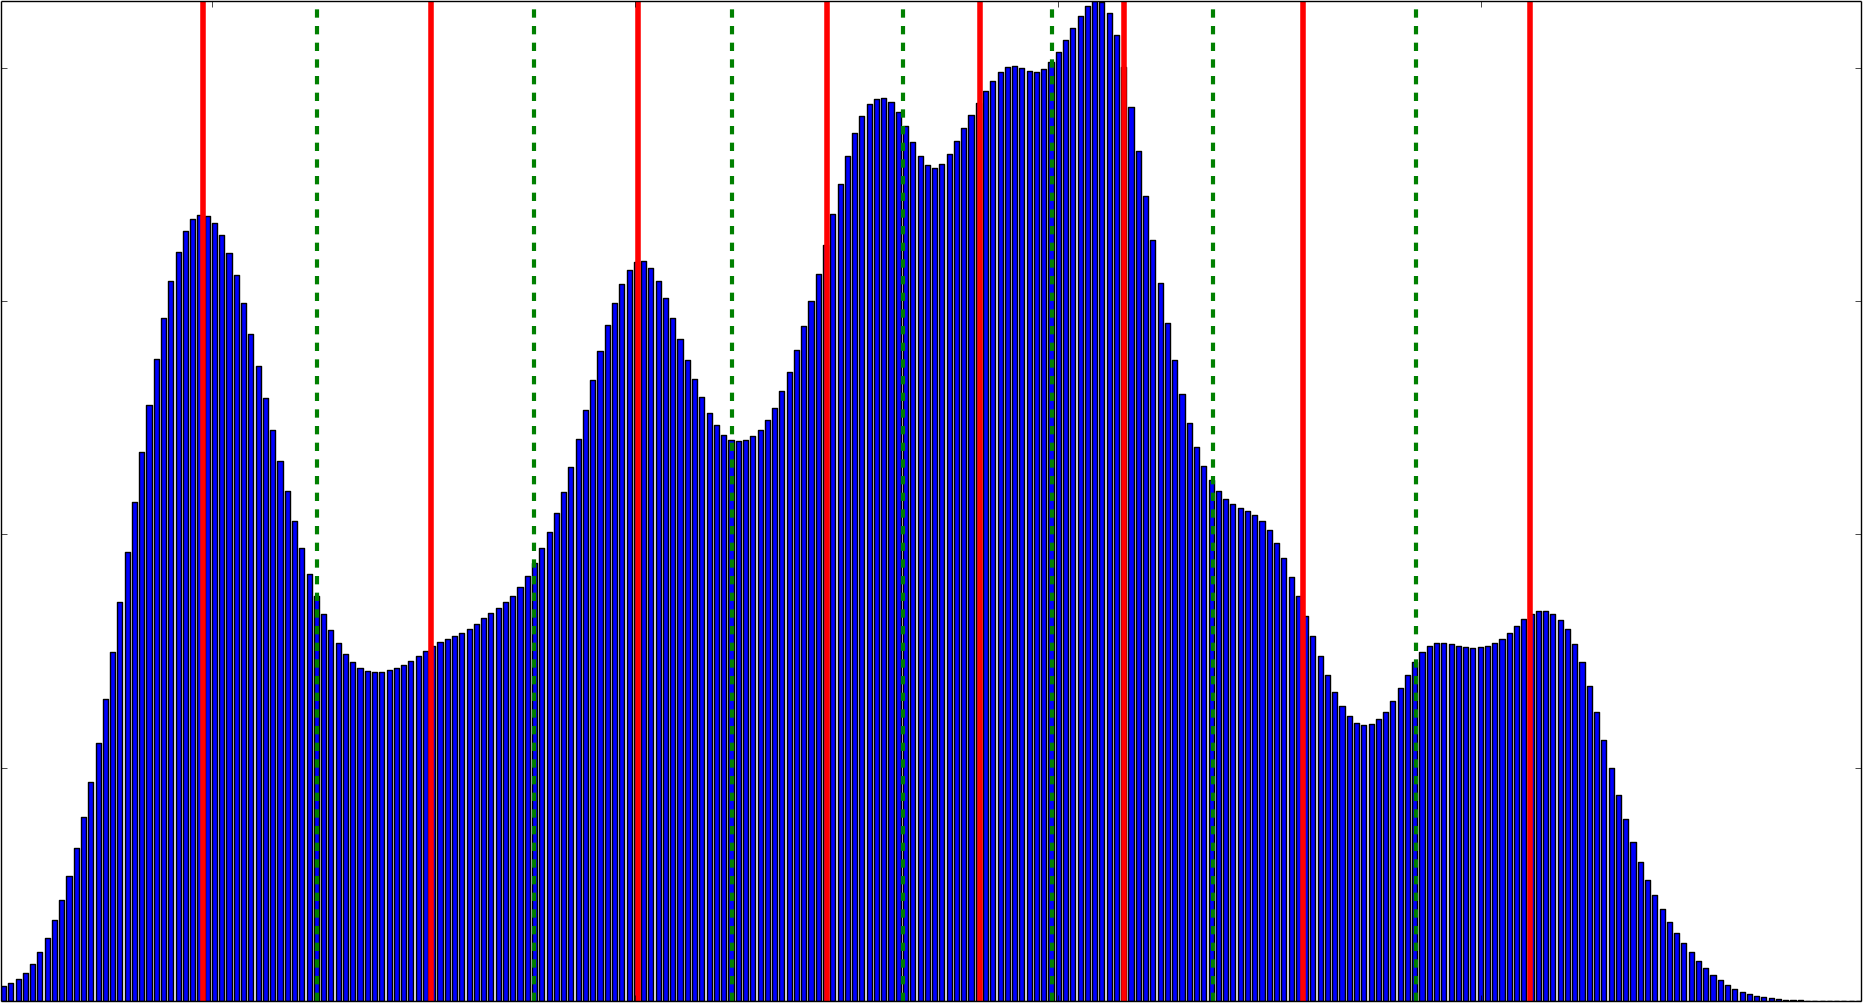
\includegraphics[width=0.7\textwidth]{FIGURES/lena_histogram_annot}}
    \end{center}
  \item For 1D features: $k$-means tries to separate the bumps in the histogram!
  \item What if $k$ is far from the number of bumps,
  \item if bumps are unclear?
  \item if bumps are very close?
  \item What makes a bump? ML course?
    \pause
\end{itemize}
\end{frame}


\begin{frame}{Example}
  \begin{center}
    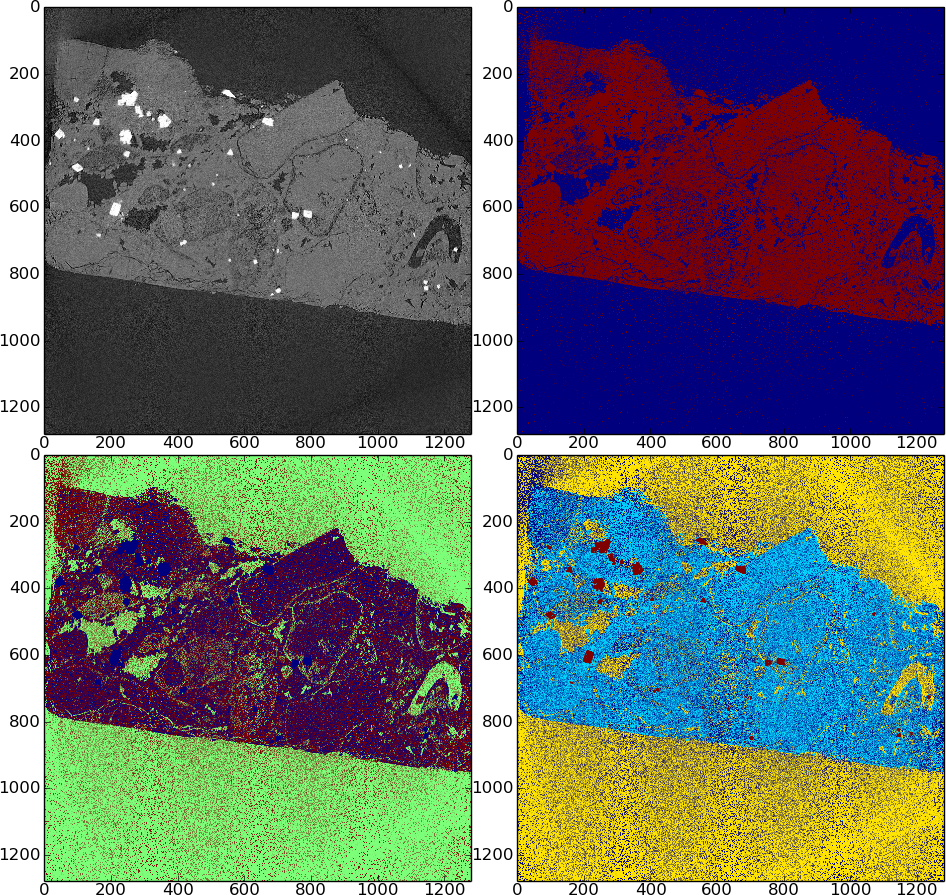
\includegraphics[width=0.6\textwidth]{FIGURES/WIG1TSegkmeans}
  \end{center}
  Original image and $k$-means clustering for $k$=2,3,4. 
\end{frame}




\begin{frame}[t]{Otsu Clustering Method -- 1979}
  \begin{itemize}
  \item For 2 regions:\vfill
    \begin{itemize}
    \item Find threshold such that \myemph{intraclass variance} is minimized
      $$
      \sigma_w(t)^2 := \omega_1(t)\sigma_1^2(t) + \omega_2(t)\sigma_2^2(t)
      $$
      \vfill
    \item $\omega_1(t) = \frac{\# \text{pixels } < t}{\#\text{pixels in image}}$ = probability that pixel value is $<t$, 
      $\omega_2(t) = \frac{\# \text{pixels } \geq t}{\#\text{pixels in image}}$ = probability that pixel value is $\geq t$.\vfill
    \item $\sigma_1^2(t) = $ variance of the class of pixels $< t$, \\
      $\sigma_2^2(t) = $ variance of the class of pixels $\geq t$, \vfill
    \item Search for $t$ in range $[\min(\text{image value}),\max(\text{image value})]$.
    \end{itemize}
    \vfill
  \item Performed on image histogram.
  \item Easily generalized to more classes/regions.
  \item Can search for local thresholds (on subimages).
  \end{itemize}
\end{frame}

\begin{frame}[t]{Example}
  \begin{center}
    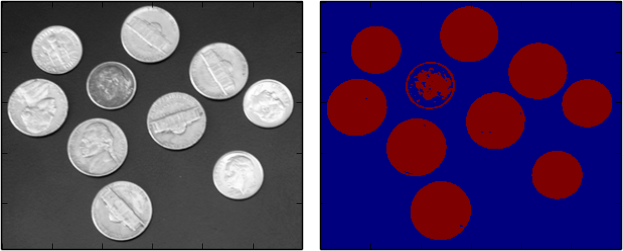
\includegraphics[width=0.7\textwidth]{FIGURES/CoinsOtsu}
  \end{center}
  \begin{center}
    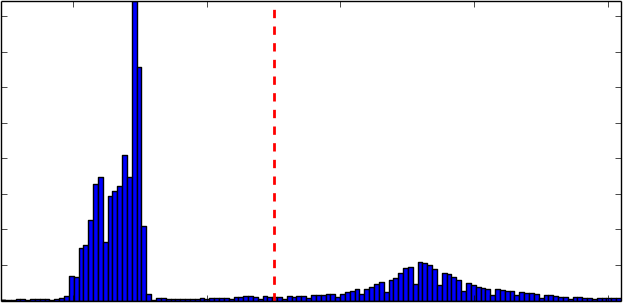
\includegraphics[width=0.7\textwidth]{FIGURES/CoinsOtsuHistogram}
  \end{center}
\end{frame}


\begin{frame}[t]{Multiple Classes Otsu}
  \begin{center}
    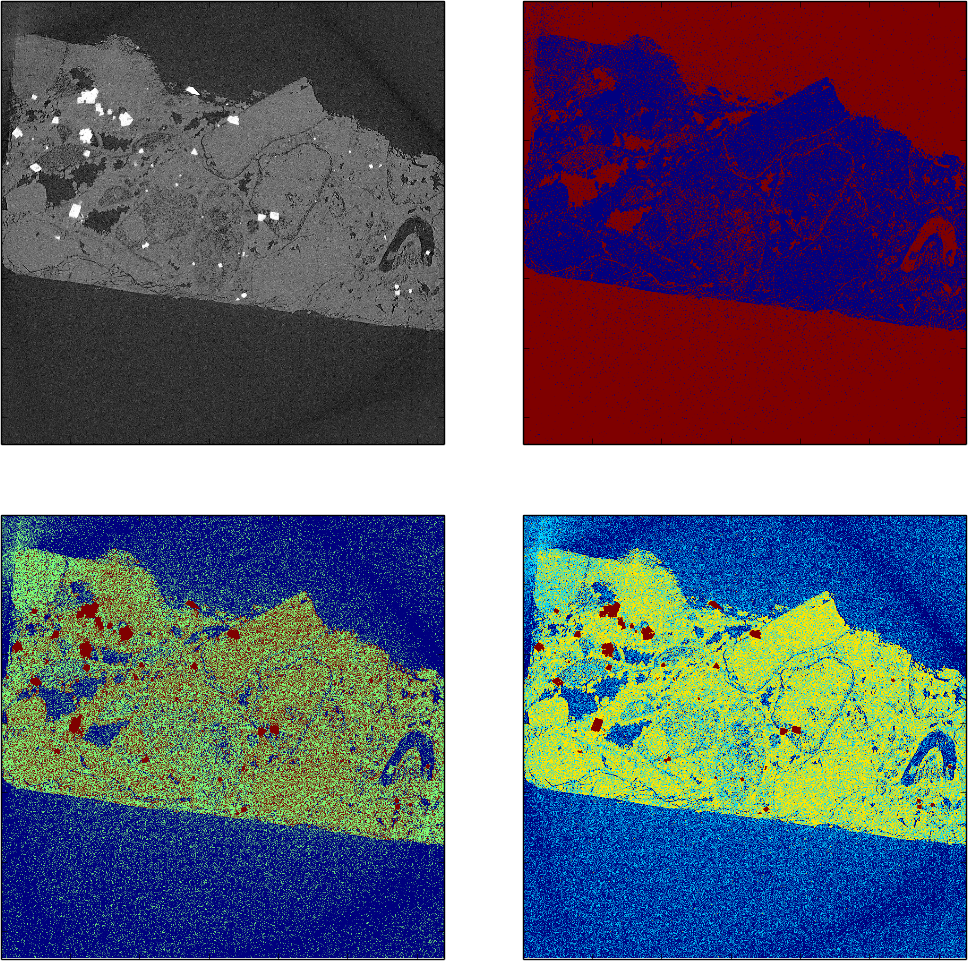
\includegraphics[width=0.5\textwidth]{FIGURES/WIG1T_Otsu}
  \end{center}
  \begin{center}
    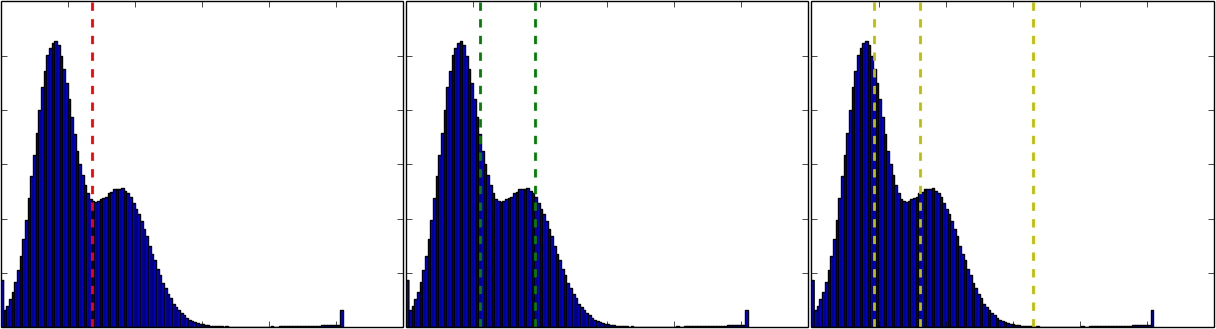
\includegraphics[width=0.7\textwidth]{FIGURES/WIG1TOtsu2Histograms}
  \end{center}
\end{frame}





\section{Spatial Regularization}


\begin{frame}[t]{Clustering and Noise}
  \begin{itemize}
  \item Intensity clustering discard does not use spatial proximity grouping
  \item Noise disturbs clustering.
  \end{itemize}
  \begin{center}
    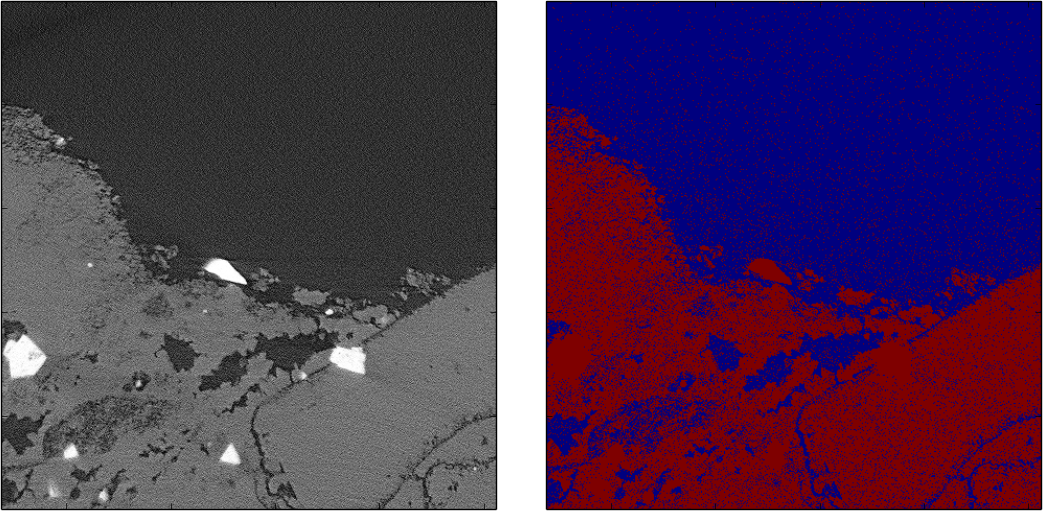
\includegraphics[width=0.9\textwidth]{FIGURES/WIG1T_OtsuNoise}\\
    ~\\
    Computed X-Ray tomography from a sandstone sample. Relatively high noise level.
  \end{center}
\end{frame}


\begin{frame}[t]{Local Spatial Coherence}
  \begin{itemize}
  \item Prevent small holes: pixel of class A surrounded by pixels of class B: remember proximity grouping.\vfill
  \item Local proximity defined in term of pixel \myemph{neighborhoods}\vfill
    \begin{center}
      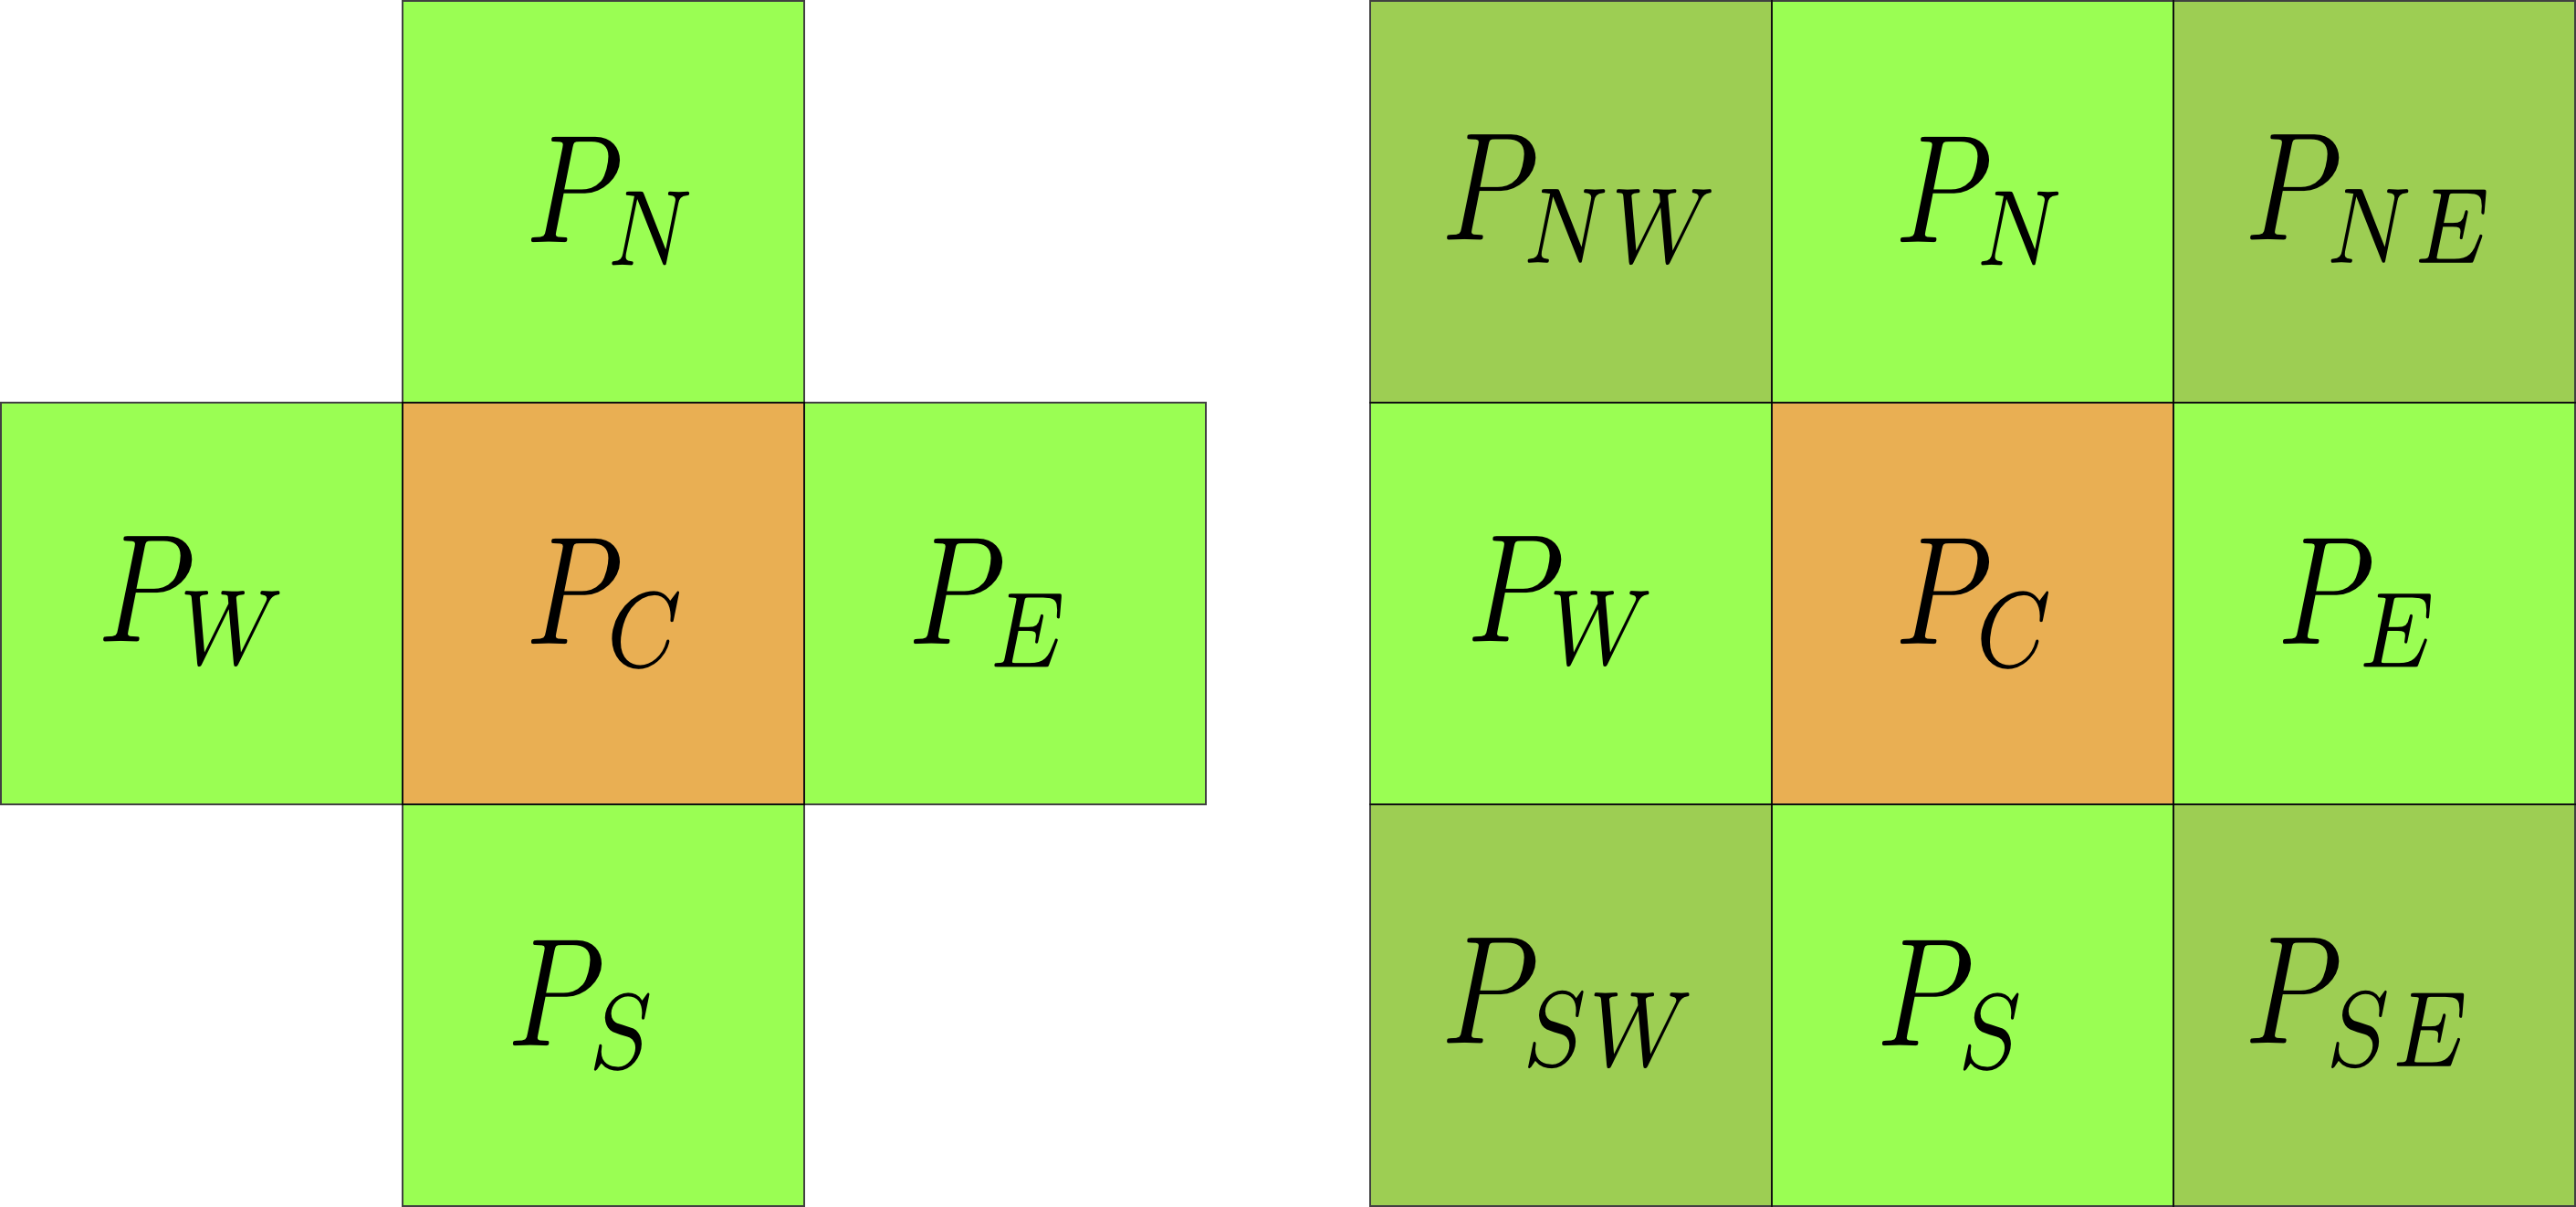
\includegraphics[width=0.7\textwidth]{FIGURES/neighborhoods}~\\
      4 and 8 pixels neighborhood systems.
    \end{center}\vfill
  \item If neighbor pixels have same (or almost same) labels, replace center pixel by dominant one.
  \end{itemize}
\end{frame}



\begin{frame}[t]{Example}
  \vfill
  \begin{center}
    \begin{tikzpicture}
      \node(img1) {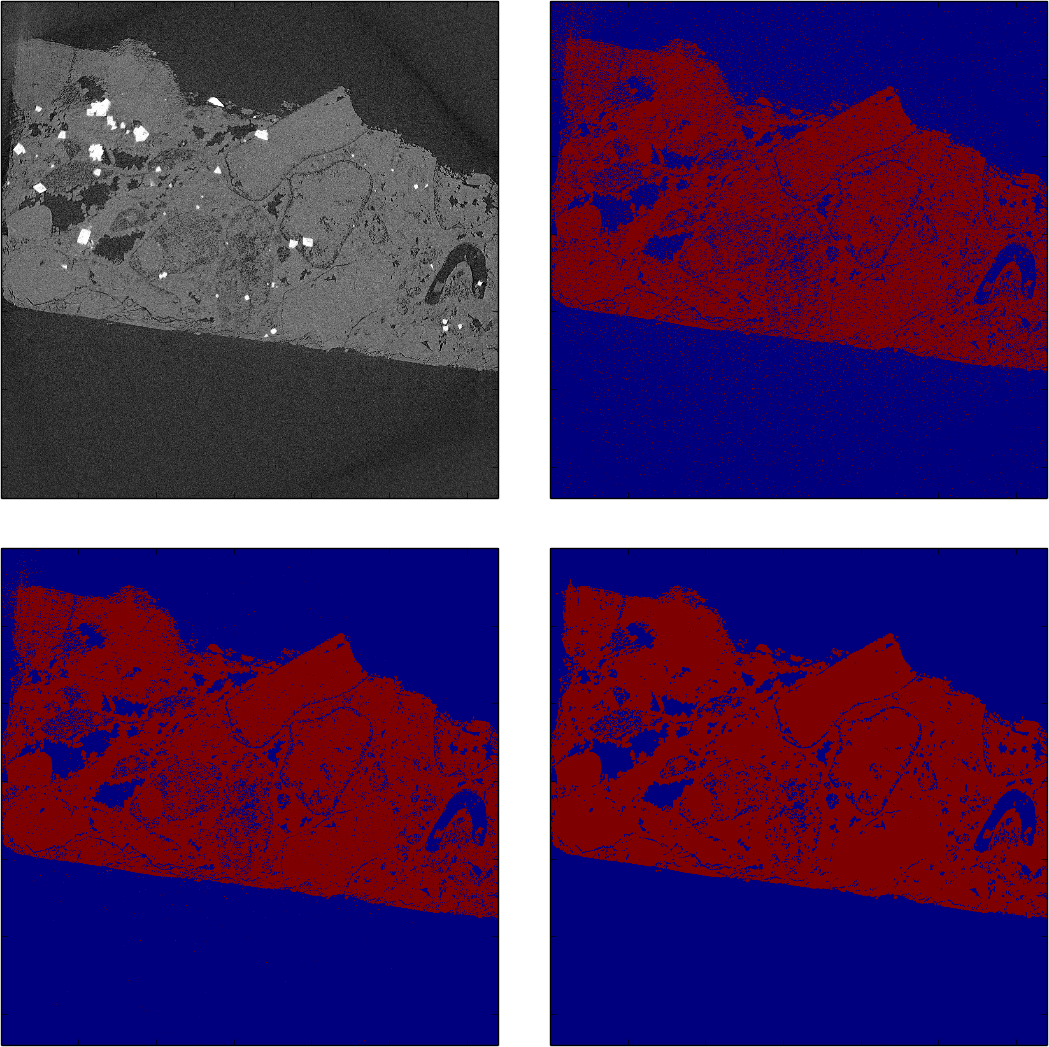
\includegraphics[width=0.6\textwidth]{FIGURES/WIG1T_RegOtsu}};
      \pause
      \node(img1) {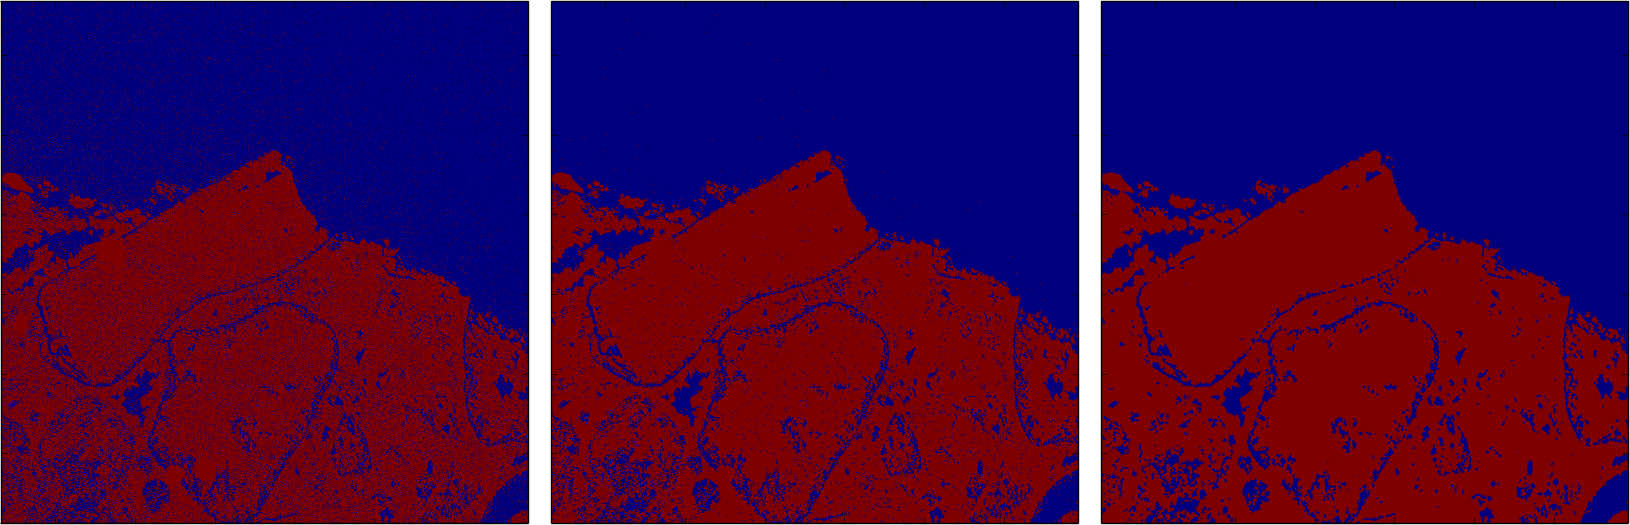
\includegraphics[width=1.1\textwidth]{FIGURES/WIG1T_RegOtsuZoom}};
    \end{tikzpicture}
    % 
    % \visible<2>{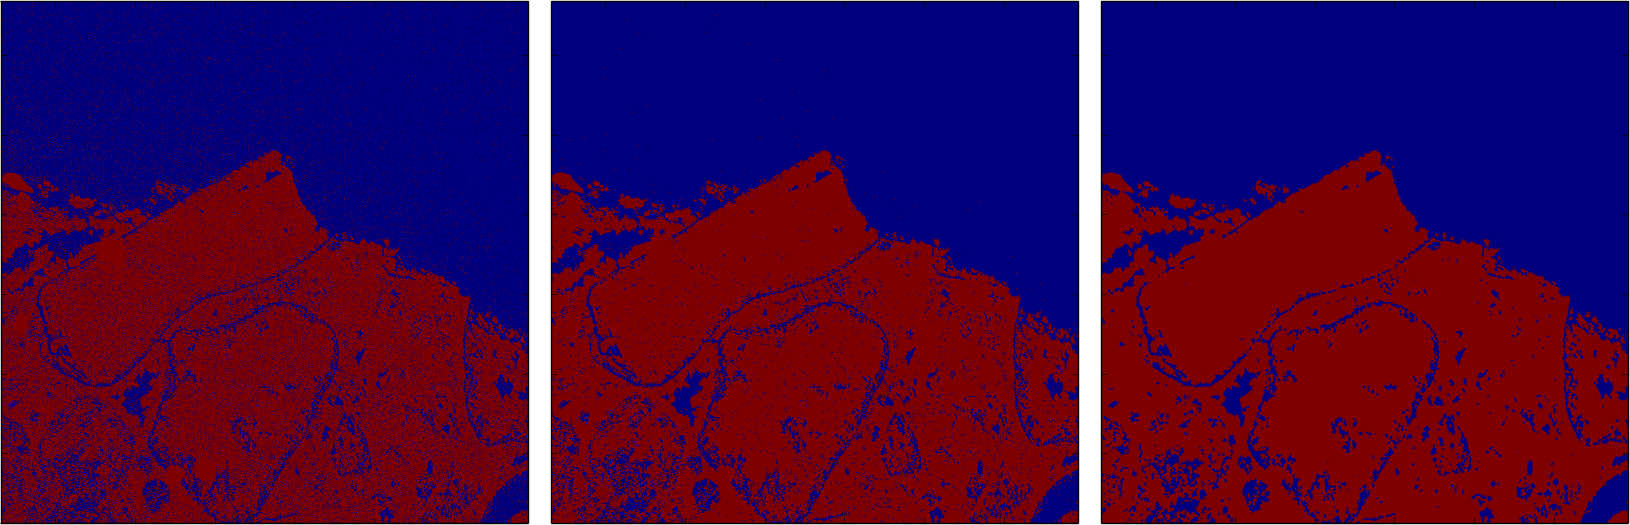
\includegraphics[width=0.7\textwidth]{FIGURES/WIG1T_RegOtsuZoom}}
  \end{center}\vfill
\end{frame}






\begin{frame}[t]{Clustering Snakes: Chan-Vese Algorithm}
  \begin{itemize}
  \item Mixes ideas: Clustering ($k$-means), Snakes a.k.a Active contours, Spatial Regularization.
  \item Performs clustering while enforcing region coherence -- remove small holes.\vfill
  \item Continuous formulation: find a curve $C$, numbers $u_0$, $u_1$ (class centroids)  minimizing
    $$
    \Ee(C,u_0,u_1) = \int_{\text{int}(C)}(u-u_0)^2\,dx + \int_{\text{ext}(C)}(u-u_1)^2\,dx +  \lambda\text{length}(C) 
    $$\vfill
  \item Minimization by solving a Partial Differential equation for $C$.\vfill
  \item Complex, non linear.\vfill
  \item Very effective implementations -- level sets, relaxations.\vfill
  \item Hundreds of derived methods.\vfill
  \end{itemize}
\end{frame}


\begin{frame}[t]{Chan Vese Example}
  \begin{center}
    \begin{tabular}[h]{ccc}
      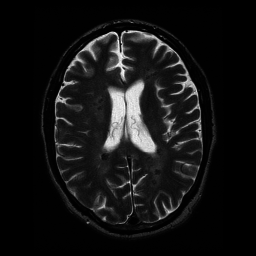
\includegraphics[width=0.25\textwidth]{FIGURES/braint2} & 
      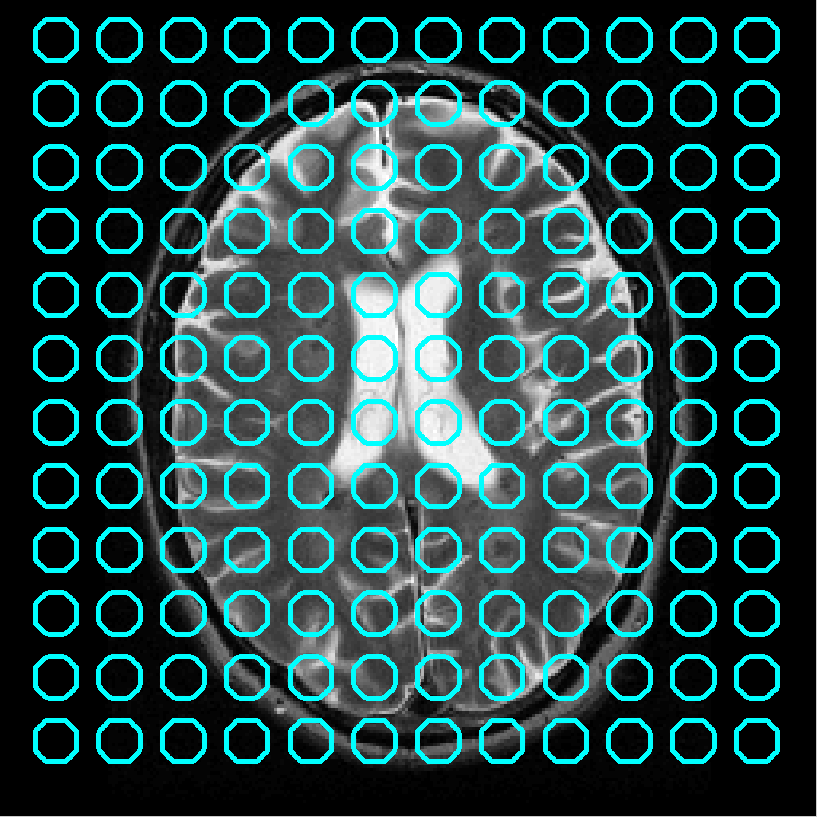
\includegraphics[width=0.25\textwidth]{FIGURES/brainseg_frame_000} &
      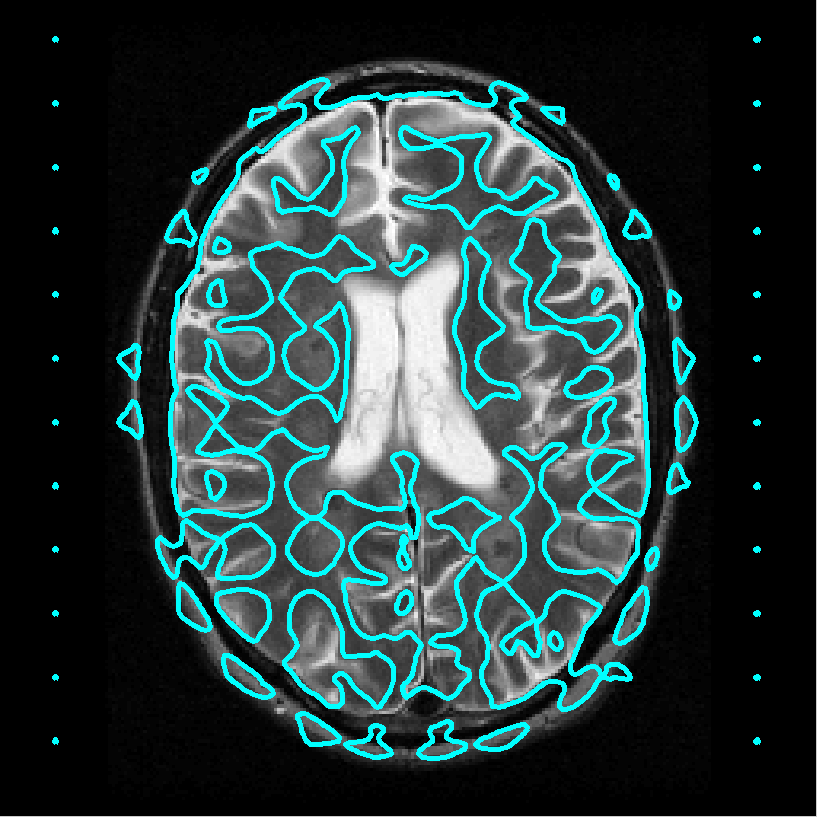
\includegraphics[width=0.25\textwidth]{FIGURES/brainseg_frame_010}\\
      \includegraphics[width=0.25\textwidth]{FIGURES/brainseg_frame_030} &
      \includegraphics[width=0.25\textwidth]{FIGURES/brainseg_frame_050} &
      \includegraphics[width=0.25\textwidth]{FIGURES/brainseg_frame_100}
    \end{tabular}
  \end{center}
\end{frame}



\section{Summary}

\begin{frame}[t]{Summary}
  \begin{center}
    {\fontsize{8}{6}\selectfont
      \begin{itemize}
      \item Ideas from Gestalt theory: Figure-Ground, grouping: proximity, connectedness, similarity, continuity, closure, common regions.
      \item Segment as ``small'' semantic unit.
      \item Edges and segmentation: Marr-Hildreth edge detector, Canny Edge detector.
      \item Closing the gap. Perceptual aspects (amodal completion), operationalization: Snakes - a.k.a. Active contours.
      \item Feature proximity, clustering, K-Means, Otsu.
      \item Noise and Gap. Spatial regularization.
      \item Chan-Vese: Clustering Snakes.
      \end{itemize}
    }
    \end{center}
    \pause
    \begin{center}
    \visible<2->{\includegraphics[width=0.5\textwidth]{IMAGES/xmastreesnake}}
  \end{center}
\end{frame}


\begin{frame}
      \includegraphics[width=1\textwidth]{IMAGES/tired}
\end{frame}



















































% %%%%%%%%%%%%%%%%%%%%%%%%%%%%%%%%%%%%%%%%%%%%%%%%%%%%%%%%%%%%
% %
% % For next session of the course:
% %
% % TO BE DONE: Write the discrete version everywhere, only 
% % mention the  continuous one with integrals!
% %
% %
% %%%%%%%%%%%%%%%%%%%%%%%%%%%%%%%%%%%%%%%%%%%%%%%%%%%%%%%%%%%%


% \begin{frame}
%   Finally, One gets an approximation of the length by
%   $$
%   \ell(C) \approx \sum_{i=1}^k |C'(p+i dp)|dp
%   $$
%   Making $dp\to 0$ one gets
%   $$
%   \ell(C) = \int_a^b |C'(p)|dp
%   $$
%   The length of $C$ is a measure of complexity of the curve. Related to the length is the \myemph{curve energy}
%   $$
%   \Ee(C) = \int_a^b |C'(p)|^2\,dp
%   $$
% \end{frame}


% \begin{frame}
%   \frametitle{Discrete Formulation}
%   \begin{itemize}
%   \item In the sequel, subtracting two points in the plane means getting the vectors joining them, and means subtracting
%     their coordinates
%     $$
%     P_1 = (4,3),\quad P_2 = (1,2),\quad P_2-P_1 = \overrightarrow{P_1P_2} = (-3,-1). 
%     $$
%     \begin{center}
%       \includegraphics[width=0.35\textwidth]{FIGURES/diffpoints}
%     \end{center}
%   \item The length of vector $P_2-P_1$ is denoted $\|P_2-P_1\|$ and is $\sqrt{(x_2-x_1)^2 + (y_2-y_1)^2}$.
%   \end{itemize}
% \end{frame}


% \begin{frame}
%   \frametitle{Curve representation}
%   \begin{itemize}
%   \item A closed curve $C$ will be represented by $n$ points $P_1,P_2,\dots,P_n$, and consecutive points are joined
%     by line segments, and with $P_{n+1} = P_1,$, $P_0=P_n$ indicating that the curve is closed: 
%     \begin{center}
%       \includegraphics[width=0.75\textwidth]{FIGURES/closedcurvepoints}\\
%       A closed curve with 12 points
%     \end{center}
%   \end{itemize}
% \end{frame}


% \begin{frame}
%   \frametitle{Discrete Snake Energy: Curve Internal Forces}
%   \begin{itemize}
%   \item Curve Energy term: sum of squared length of the curve segments:
%     $$
%     E_\Cc(C) = \sum_{i=1}^n\|P_{i+1}-P_i\|^2,\quad P_{n+1} = P_1.
%     $$
%   \item Bending energy term: sum squared-length of  differences of consecutive segments
%     \begin{align*}
%       E_\Bb(C) &= \sum_{i=1}^n\| (P_{i+1}-P_i) - (P_i-P_{i-1})\|^2\\
%       &=\sum_{i=1}^n\| P_{i+1}-2P_i+P_{i-1}\|^2,\quad P_{n+1} = P_1, P_0 = P_n.
%     \end{align*}
%   \end{itemize}
% \end{frame}



% \begin{frame}
%    \frametitle{Discrete Snake Energy: External (Image) Forces}
%    \begin{itemize}
%    \item
%      $F$ is an image derived from the image $I$ to be segmented, with the property that
%      $F$ should be small when at an edge of $I$ and large when at a flat region of $I$. 
%    \item Standard example is 
%      $$
%      F = -\|\nabla I_\sigma\|^2 = -\left(I_{\sigma x}^2 + I_{\sigma y}^2\right)^2.
%      $$
%      with $I_\sigma = g_\sigma\ast I$, $I$ convolved with Gaussian of standard deviation $\sigma$.
%    \item External force at point $P = (x,y)$: $F(P) = F(x,y)$ and external / image energy:
%      $$
%      E_\Ee(C) = \sum_{i=1}^n F(P_i).
%      $$
%    \end{itemize}
%  \end{frame}



%  \begin{frame}
%    \frametitle{External Forces: Example}
%    \begin{itemize}
%    \item Using the force term $F= -\|\nabla I_\sigma\|^2$, dark indicates edge:
%      \begin{center}
%        \begin{tabular}[h]{cc}
%           \includegraphics[width=0.45\textwidth]{IMAGES/coins} & 
%           \includegraphics[width=0.45\textwidth]{IMAGES/cannyextcoins} \\
%           Original image & Force term with $\sigma = 3$
%        \end{tabular}
%      \end{center}
%    \end{itemize}
%  \end{frame}

%  \begin{frame}
%    \frametitle{Snake Energy}
%    \begin{itemize}
%    \item Given a discrete closed curve $C = (P_1,P_2,\dots,P_n)$, its Snake Energy is 
%      \begin{align*}
%        E_\Ss(C) &= \alpha E_\Cc(C) + \beta E_\Bb(C) + \gamma E_\Ee(C)\\
%        &= \alpha\sum_{i=1}^n\|P_{i+1}\!-P_i\|^2 \!\!+ \beta\sum_{i=1}^n\|P_{i+1}\!-2P_i+p_{i-1}\|^2 \!\!+ \gamma\sum_{i=1}^n F(P_i)\\
%        &=\sum_{i=1}^n\left(\alpha\|P_{i+1}-P_i\|^2+\beta\|P_{i+1}-2P_i+P_{i-1}\|^2+\gamma F(P_i)\right).
%      \end{align*}
%    \item $\alpha$, $\beta$ and $\gamma$ are 3 weights (i.e., positive numbers) that
%      provide the trade-off between the different parts.
%    \end{itemize}
%  \end{frame}



% \begin{frame}
%   \frametitle{With Coordinates}
%   \begin{itemize}
%   \item $C = (P_1,\dots,P_n) = ((x_1,y_1),\dots,(x_n,y_n)) \rightsquigarrow (x_1,\dots,x_n,y_1\dots,y_n)$
%   \item $E_\Ss(C) = E_\Ss(x_1,\dots,x_n,y_1, \dots,y_n)$
%     \begin{multline*}
%       E_\Ss(C) = \alpha\sum_{i=1}^n\left((x_{i+1}-x_i)^2 + (y_{i+1}-y_i)^2\right)+\\
%       \beta\sum_{i=1}^n\left((x_{i+1}-2 x_i + x_{i-1})^2 + (y_{i+1}-2 y_i + y_{i-1})^2\right)
%     \end{multline*}
%     We assume that $x_{i+1} = x_1$, $y_{i+1} = y_1$ (closed curve).
%   \item $E_\Ee(C) = E_\Ee(x_1,\dots,x_n,y_1, \dots,y_n)$
%     $$
%     E_\Ee(C) = \sum_{i=1}^n F(x_i,y_i)
%     $$
% \end{itemize}
% \end{frame}

% \begin{frame}
%   \frametitle{Gradient}
%   \begin{itemize}
%   \item $\nabla_C \Ee = \left(\pder{E}{x_1},\dots,\pder{E}{x_n},\pder{E}{y_1},\dots,\pder{E}{y_n}\right)^T$
%   \item Smoothness term:
%     $$
%     \pder{E_\Ss}{x_i} = -2\alpha\left(x_{i+1}-2x_i+x_{i-1}\right) + ...
%     $$
%   \item remaining computations left as an exercise!
%   \end{itemize}
% \end{frame}


% % \begin{frame}
% %   \frametitle{Stiffness - Complexity measure of the curve.}
% %   \begin{itemize}
% %   \item  Winding can be measure by the \myemph{bending energy}:
% %     $$
% %     \Ss(C) = \int_a^b|C''(p)|^2\,dp
% %     $$
% %     We have used the second derivative $C''$ of the curve.
% %   \item
% %     Put it together:
% %     $$
% %     E_R(C,\alpha,\beta) = \alpha\Ee(C) + \beta\Ss(C)
% %     $$
% %     gives a combination of the curve energy and its
% %     bending energy. $\alpha$ and $\beta$ control the ratio between the
% %     curve energy and the bending energy in the regularity measure.
% %   \item A sufficiently \emph{simple} curve should have a low
% %     complexity measure $E(C,\alpha,\beta)$.
% %   \end{itemize}

% % \end{frame}


% % \section{Snakes}

% % \begin{frame}
% %   \frametitle{Segmentation via Snakes} Kass, Witkin, Terzopoulos
% %   (1988) model a boundary as a close curve and put the following
% %   requirements
% %   \begin{enumerate}
% %   \item The curve should follow the edges.\vfill
% %   \item the curve should be simple as defined above.
% %   \end{enumerate}
% % \end{frame}

% % \begin{frame}
% %   \frametitle{Snakes}
% %   \begin{itemize}
% %   \item The curve should follow edges of image $f$: for instance
% %     $|\nabla f(C(p))|^2$ should be as large as possible since high
% %     gradients can be edge indicators and $|\nabla f(C(p))|^2$ should
% %     be as small as possible.Let $F(f,C(p))$ a function such that
% %     $F(f,C(p))$ small when $C(p)$ on image edge.
% %     $$
% %     e(C) = -\int_0^1F(f,C(p)),dp
% %     $$
% %   \item $F$ could use a smoothed gradient of $f$
% %   \item Snake approach: Find a curve $C$ which \myemph{minimizes} the \myemph{Snake energy}
% %     $$
% %     E_{S}(C) = \alpha\int_0^1|C'(p)|^2 dp + \beta\int_0^1|C''(p)|^2 dp +\gamma
% %     \int_0^1F(f,C(p))\,dp.
% %     $$
% %   \item Solving the problem is an example of the \myemph{Calculus of Variations}.
% %   \end{itemize}
% % \end{frame}


% % \begin{frame}
% %   \begin{itemize}
% %   \item For functionals i.e. Functions of functions: the same.
% %   \item Snakes: Embed $C(p)$ in family of curves $C(p,t)$, $C(p,0)$ is the starting curve.
% %   \item Evolve by 
% %     $$
% %      \pder{C(-,t)}{t} = -\nabla_{C(-,t)} E_S
% %     $$
% %   \item Gradient of $E_S$: How can we compute that thing?
    
% %   %   the left-hand-side of Euler-Lagrange Equation.
% %   % \item Descent becomes:
% %   %   $$
% %   %    \pder{C(-,t)}{t} = \alpha \pderd{2}{C(p,t)}{p^2} - \beta \pderd{4}{C(p,t)}{p^4} +\lambda \nabla_{C(p,t)}F
% %   %    $$
% %   \end{itemize}  
% % \end{frame}


% % \begin{frame}
% %   \begin{itemize}
% %   \item A curve minimizing $E_S$ should be a zero of the gradient of $E_S$.
% %   \item But a curve is not a real number or a vector! So we cannot use
% %     the standard rules of differential calculus. 
% %   \item Idea (\myemph{absolutely fundamental}): perturb $C$ by
% %     a ``closed curve'' $D : [0,1]\to\RR^2$ i.e., replace $C$ by $C+ tD
% %     : p\mapsto C(p) + tD(p)$.
% %     $$
% %     \ell(t) = \Ee(C + t D)
% %     $$
% %     If $C$ minimizes $E_S$, $\ell'(0)$ should be 0 for every reasonable $D$. This gives (details omitted...)
% %     $$
% %     -\alpha C''(p) + \beta C^{(4)}(p) -\gamma \nabla_{C(p)}F = 0,\quad \forall p.
% %     $$
 
% %   \end{itemize}
% % \end{frame}

% % \begin{frame}
% %   \begin{itemize}
% %   \item This is in fact the combination of two equations, for the $x$ and $y$ coordinates of the curve:
% %     \begin{align*}
% %       -\alpha x''(p) + \beta x^{(4)} +\gamma \pder{F}{x}(x(p),y(p)) &=0\\
% %       -\alpha y''(p) + \beta y^{(4)} +\gamma \pder{F}{y}(x(p),y(p)) &=0
% %     \end{align*}
% %   \item This is a example of \myemph{Euler-Lagrange equation}
% %   \item the term 
% %     $$
% %     -\alpha C''(p) + \beta C^{(4)}(p) +\gamma \nabla_{C(p)}F
% %     $$
% %     is the gradient of $E_S$.
% %   \end{itemize}
% % \end{frame}






% \begin{frame}
%   \frametitle{Snake example}
%   \begin{center}
%     \includegraphics[width=0.4\textwidth]{IMAGES/heartgac}
%   \end{center}
%   Segmentation of heart using a variant of Snakes by A. Tatu,
%   F. Lauze, S. Sommer and N. Nielsen. External contour is the initial
%   one. Internal after convergence.
% \end{frame}

% %---------------------------------------------------------------------


% \section{Numerical tools for Snakes implementation}





% \begin{frame}
%   \frametitle{Gradient Descent}
%   \begin{itemize}
%   \item $\bar{x}$ minimizes $f(x)$, $f$ differentiable: $\nabla_{\bar{x}} f = 0$
%   \item Gradient indicates the direction to take so as make the
%     function increase most. For the opposite (i.e., getting to a
%     minimum): follow $-\nabla f$
%     \begin{center}
%       \includegraphics[width=0.7\textwidth]{FIGURES/graddesc}
%     \end{center}
%   \item Descent: Take small, steps in the direction indicated by $-\nabla f$:
%     embed an original estimate $x_0$ in a family of
%     points $x_i$ (or $x(t)$ for a continuous formulation)
%     $$
%     x_{i+1} = x_i - \tau\nabla_{x_i}F,\quad \tder{}{x}{t} = -\nabla_{x(t)}f
%     $$
%   \end{itemize}
% \end{frame}


% \begin{frame}
%   \frametitle{Simple Example -- Explicit Scheme}
%   \begin{itemize}
%   \item $F(x) = x^2$. $\nabla_x F = F'(x) = 2x$. Minimum for $x = 0$.
%   \item Gradient descent:
%     $$
%     x_{i+1} = x_i - \tau F'(x_i) = x_i - 2\tau x_i = (1-2\tau)x_i
%     $$
%   \item If $\tau$ too large, problems: try with $\tau = 1$!
%   \item If $\tau < 1/2$, decreasing sequence.
%   \item If $\tau = 1/2$, converges in 1 step! 
%   \end{itemize}
% \end{frame}

% \begin{frame}
%   \frametitle{Nonlinear Problem}
%   \begin{itemize}
%   \item $F(x) = F(x_1,\dots,x_n) = \|x\|$, $x\in\RR^n$, $\|x\| = \sqrt{x_1^2+\dots x_n^2}$.
%   \item Minimum at $x = (0,\dots,0)$.
%   \item Gradient of $F$: 
%     $$
%     \nabla_x F = 
%     \begin{pmatrix}
%       \pder{F}{x_1}\\
%       \vdots\\
%       \pder{F}{x_n}
%     \end{pmatrix}
%     =
%     \begin{pmatrix}
%       \frac{x_1}{\|x\|}\\
%       \vdots\\
%       \frac{x_n}{\|x\|}
%     \end{pmatrix}
%     =
%     \frac{x}{\|x\|}
%     $$
%     \item Explicit descent:
%       $$
%       x_{i+1} = x_i -\tau \frac{x_i}{\|x_i\|} = x_i\left(1-\frac{\tau}{\|x\|}\right)
%       $$
%     \item If $\tau > \|x_i\|$, $1-\frac{\tau}{\|x\|} < 0$, oscillating!
%   \end{itemize}
% \end{frame}


% \begin{frame}
%   \frametitle{Semi-implicit scheme}
%   \begin{itemize}
%   \item $\nabla_x F = \frac{x}{\|x\|}$ is complex, several ways to deal with it in descent.
%   \item Instead of explicit scheme, \myemph{semi-implicit}:
%     $$
%     x_{i+1} = x_i -\tau\frac{x_{i+1}}{\|x_i\|}
%     $$
%   \item Provides descent scheme:
%     $$
%     x_{i+1} = \frac{x_i}{1+ \tau\|x_i\|}
%     $$
%   \item Will never oscillate!
%   \item If possible, use a semi-implicit scheme instead of an explicit one.
%   \end{itemize}
% \end{frame}

% % \begin{frame}
% %   \frametitle{How to approximate derivatives of curves numerically?}
% %   \begin{itemize}
% %   \item Numerically we are given a set of points $C_1\dots C_N$ in the plane (i.e.) the set of their coordinates.
% %   \item First order derivative:
% %     $$
% %     C'_i \approx \frac{C_{i+1}-C_{i-1}}{2}
% %     $$
% %     It comes from the formula
% %     $$
% %     C'(p) =\lim_{dp\to 0}\frac{C(p+dp)-C(p-dp)}{dp}
% %     $$
% %     with $dp = 1$ (the distance between the curve parameter samples). 
% %   \end{itemize}
% % \end{frame}

% % \begin{frame}
% %   \frametitle{Higher order derivatives}
% %   We need derivatives of the curve at order 2 and 4:
% %   \begin{itemize}
% %   \item Order 2:
% %     $$
% %     C''_i \approx C_{i-1} - 2C_i + C_{i+1}
% %     $$
% %     It comes from the formula
% %     $$
% %     C''(p) =\lim_{dp\to 0}\frac{C(p+dp) -2C(p) + C(p-dp)}{dp^2}
% %     $$
% %   \item Order 4: apply order 2 twice:\pause
% %    $$
% %     C^{(4)}_i \approx C_{i-2} - 4C_{i-1} + 6 C_i -4C_{i+1} -C_{i+2}.
% %     $$
% %     \pause
% %   \item  Note that I may have a problem when $i<=0$ of $i > N$ since I have just $N$ points  $C_1,\dots,C_N$.
% %   \item But if I have assumed that the curve is closed (and I will),  \myemph{I will take} $C_0 = C_N$, $C_{-1} = C_{N-1}$, \dots
% %   \end{itemize}
 
 
% % \end{frame}


% % \begin{frame}
% %   \frametitle{Putting it together}
% %   I want to discretize the gradient descent equation: 
% %   $$
% %   \pder{C(-,t)}{t} = \alpha C'' - \beta C^{(4)} -\gamma \nabla_C F
% %   $$
% %   \begin{itemize}
% %   \item Call $C^n$ the curve after $n$ evolutions of descent. The left hand side at point $C_i$ can be approximated by 
% %     $$
% %      \pder{C_i(t)}{t} \approx \frac{C_i^{n+1} - C_i^n}{\tau}
% %     $$
% %     with $\tau$ a small \myemph{time-step}
% %   \end{itemize}
% % \end{frame}

% % %%%%%%%%%%%%%%%%%%%%
% % %%%% CHECK IT!!!!!!
% % %%%%%%%%%%%%%%%%%%%%
% % \begin{frame}
% %   \begin{itemize}
% %   \item The right-hand side, omitting the external force gradient, can be written as 
% %     \begin{align*}
% %      \alpha\left(C_{i-1} - 2C_i + C_{i+1}\right) - \beta\left(C_{i-2} - 4C_{i-1} + 6 C_i -4C_{i+1} -C_{i+2}\right)\\
% %      = -\beta C_{i-2} + (\alpha + 4\beta)C_{i-1} - (2\alpha + 6\beta)C_i +(\alpha + 4\beta)C_{i+1} - \beta C_{i+1}
% %     \end{align*}
% %   \item Call the above quantity $L(\alpha,\beta,i)C$, the discrete descent can be written in a shorter form as
% %     $$
% %       \frac{C_i^{n+1}-C_i^{n}}{\tau} = L(\alpha,\beta)C^n -\gamma\nabla_{C_i^n}F
% %     $$
% %   \item This gives a solution as
% %     $$
% %     C_i^{n+1} = C_i^{n} - \tau\left(L(\alpha,\beta,i)C^n -\gamma\nabla_{C_i^n}F\right)
% %     $$
% %   \item This is called an explicit scheme, and is fairly easy to
% %     implement once on can compute $\nabla_C F$.
% %   \end{itemize}  
% % \end{frame}


% % \begin{frame}
% %   \frametitle{Implicit scheme I} 
% %   \begin{itemize}
% %   \item The above equation has the drawback to
% %     work only for rather small $\tau$s. Instead one can use a so called
% %     \emph{(semi-)implicit scheme}:
% %     $$
% %      \frac{C_i^{n+1}-C_i^{n}}{\tau} = L(\alpha,\beta,i)C^{n+1} -\gamma\nabla_{C_i^n}F
% %     $$
% %   \item The difference is subtle, can you spot it?\pause
% %   \item Look at the explicit scheme equation:
% %      $$
% %       \frac{C_i^{n+1}-C_i^{n}}{\tau} = L(\alpha,\beta)C^n -\gamma\nabla_{C_i^n}F
% %     $$\pause
% %   \item In the implicit scheme, I use a future value of the curve in the right-hand-side!
% %     Weird, I have not yet computed it! But...
% %   \end{itemize}
% % \end{frame}

% % \begin{frame}
% %   \frametitle{Implicit scheme II}
% %   \begin{itemize}
% %   \item We unroll the equation:
% %     $$
% %     C^{n+1}_i - \tau L(\alpha,\beta,i)C^{n+1} = C_i^n - \tau\gamma\nabla_{C_i^n}F
% %     $$
% %   \item This gives{\small
% %       \begin{multline*}
% %         \tau\beta C^{n+1}_{i-2} - \tau(\alpha+4\beta)C_{i-1}^{n+1} + (1+\tau(2\alpha+ 6\beta))C_i^{n+1} -\tau(\alpha+4\beta)C_{i+1}^{n+1} +\tau\beta C_{i+2}^{n+1} \\
% %         =C_i^n - \tau\gamma\nabla_{C_i^n}F
% %       \end{multline*}}
% %   \item All the elements of the right-hand side are known, the unknown
% %     are in the left-hand side.  I have $N$ equations of that kind, one
% %     per point in the curve and $N$ unknown values.  And each equation
% %     uses 5 unknown points values.  To compute an update of the curve, I
% %     need to solve these $N$ equations simultaneously, .
% %   \item This seems unnecessarily complicated... This is not!  The
% %     system to solve is linear, and can be rewritten as a matrix equation
% %     $$
% %     M \bx = \by.
% %     $$
% %   \end{itemize}
% % \end{frame}

% % \begin{frame}
% %   \frametitle{Implicit scheme III}
% %   Set $A = \tau\beta$, $B = -\tau(\alpha + 4\beta)$, $C = 1+ \tau(2\alpha + 6\beta)$,
% %   Here is the matrix of the linear system for a curve represented by  10 points.
% %   {\small $$ M = 
% %     \begin{pmatrix}
% %       C & B & A & 0 & 0 & 0 & 0 & 0 & A & B \\
% %       B & C & B & A & 0 & 0 & 0 & 0 & 0 & A \\
% %       A & B & C & B & A & 0 & 0 & 0 & 0 & 0 \\
% %       0 & A & B & C & B & A & 0 & 0 & 0 & 0 \\
% %       0 & 0 & A & B & C & B & A & 0 & 0 & 0 \\
% %       0 & 0 & 0 & A & B & C & B & A & 0 & 0 \\
% %       0 & 0 & 0 & 0 & A & B & C & B & A & 0 \\
% %       0 & 0 & 0 & 0 & 0 & A & B & C & B & A \\
% %       A & 0 & 0 & 0 & 0 & 0 & A & B & C & B \\
% %       B & A & 0 & 0 & 0 & 0 & 0 & A & B & C \\
% %     \end{pmatrix}
% %     $$}
% %   Note the values at the upper-right and lower down corners. This is
% %   because we deal with closed curves.
% % \end{frame}



% % \begin{frame}
% %   \frametitle{Implicit scheme III}
% %   \begin{itemize}
% %   \item  Solving the snake evolution system means solving the 2 systems for the N points
% %     \begin{columns}
% %       \column{0.49\textwidth}
% %       {\small $$ M 
% %         \begin{pmatrix}
% %           x^{n+1}_1\\x^{n+1}_2\\\vdots\\x^{n+1}_N
% %         \end{pmatrix}
% %         = \begin{pmatrix}
% %           x^{n}_1 - \gamma\pder{F}{x}(x_1^{n},y_1^{n})\\
% %           x^{n}_2 - \gamma\pder{F}{x}(x_2^{n},y_2^{n})\\
% %           \vdots\\
% %           x^{n}_N - \gamma\pder{F}{x}(x_N^{n},y_N^{n})\\
% %         \end{pmatrix}
% %         $$}
% %       \column{0.49\textwidth} 
% %       {\small $$ M 
% %         \begin{pmatrix}
% %           y^{n+1}_1\\y^{n+1}_2\\\vdots\\y^{n+1}_N
% %         \end{pmatrix}
% %         = \begin{pmatrix}
% %           y^{n}_1 - \gamma\pder{F}{y}(x_1^{n},y_1^{n})\\
% %           y^{n}_2 - \gamma\pder{F}{y}(x_2^{n},y_2^{n})\\
% %           \vdots\\
% %           y^{n}_N - \gamma\pder{F}{y}(x_N^{n},y_N^{n})\\
% %         \end{pmatrix}
% %         $$}
% %     \end{columns}
% %   \item  The matrix $M$ is invertible for all $\alpha > 0$, $\beta > 0$ and
% %     $\tau > 0$. Its inverse can be easily precomputed (Matlab
% %     \texttt{inv}, Python \texttt{numpy.linalg.inv}) for instance.
% %   \item So after all, not too complicated! And we get a probably
% %     faster scheme as potentially more stable than the simple one (Von Neumann stability analysis...)
% %   \end{itemize}
% % \end{frame}

%  \begin{frame}
%   \frametitle{Solving the segmentation}
%   {\small
%     \begin{itemize}
%      \item This is done iteratively by moving the current estimate $C^s = (P_1^s =
%        (x_1^2,y_1^s), P_2^s = (x_2^2,y_2^s),\dots, P_n^n = (x_n^s,y_n^s))$ of the contour to
%        the next one $C^{s+1} = (P_1^{s+1},P_2^{s+1},\dots,P_n^{s+1})$ in such a way that the
%        snake energy decreases most.  This needs small steps.
%      \item The theory shows that a solution can be described as solution of the systems of
%        linear equations
%      \end{itemize}
%    }
%    \begin{columns}
%      \column{0.47\textwidth}
%      {\small $$ M 
%        \begin{pmatrix}
%          x^{s+1}_1\\x^{s+1}_2\\\vdots\\x^{n+1}_N
%        \end{pmatrix}
%        = \begin{pmatrix}
%          x^{s}_1 - \gamma F_x(x_1^{s},y_1^{s})\\
%          x^{s}_2 - \gamma F_x(x_2^{s},y_2^{s})\\
%          \vdots\\
%          x^{s}_n - \gamma F_x(x_n^{s},y_n^{s})\\
%        \end{pmatrix}
%        $$}
%      \column{0.47\textwidth} 
%      {\small $$ M 
%        \begin{pmatrix}
%          y^{s+1}_1\\y^{s+1}_2\\\vdots\\y^{s+1}_N
%        \end{pmatrix}
%        = \begin{pmatrix}
%          y^{s}_1 - \gamma F_y(x_1^{s},y_1^{s})\\
%          y^{s}_2 - \gamma F_y(x_2^{s},y_2^{s})\\
%          \vdots\\
%          y^{s}_n - \gamma F_y(x_n^{s},y_n^{s})\\
%        \end{pmatrix}
%        $$}
%    \end{columns}
%    {\small
%      \begin{itemize}
%      \item $F_x$ and $F_y$ are the $x-$ and $y-$derivatives of the external force $F$, described later
%      \item $M$ is the system matrix (coefficients of the systems of equations) described
%        in an example in the slide next to the following one.
%      \end{itemize}
%    }
%  \end{frame}
 
%  \begin{frame}
%    \begin{itemize}
%    \item Solving the system of equations of the previous slide means to compute the new
%      values $x_i^{s+1}$ and $y_i^{s+1}$ as follows:
%    \end{itemize}
%    \begin{columns}
%      \column{0.47\textwidth}
%      {\small $$
%        \begin{pmatrix}
%          x^{s+1}_1\\x^{s+1}_2\\\vdots\\x^{n+1}_N
%        \end{pmatrix}
%        = M ^{-1} \begin{pmatrix}
%          x^{s}_1 - \gamma F_x(x_1^{s},y_1^{s})\\
%          x^{s}_2 - \gamma F_x(x_2^{s},y_2^{s})\\
%          \vdots\\
%          x^{s}_n - \gamma F_x(x_n^{s},y_n^{s})\\
%        \end{pmatrix},
%        $$}
%      \column{0.47\textwidth} 
%      {\small $$ 
%        \begin{pmatrix}
%          y^{s+1}_1\\y^{s+1}_2\\\vdots\\y^{s+1}_N
%        \end{pmatrix}
%        = M^{-1} \begin{pmatrix}
%          y^{s}_1 - \gamma F_y(x_1^{s},y_1^{s})\\
%          y^{s}_2 - \gamma F_y(x_2^{s},y_2^{s})\\
%          \vdots\\
%          y^{s}_n - \gamma F_y(x_n^{s},y_n^{s})\\
%        \end{pmatrix}
%        $$}
%    \end{columns}
%    \begin{itemize}
%    \item $M^{-1}$ is the \myemph{inverse matrix} of $M$.
%    \item This is the same matrix for both the abscissas and ordinates.
%    \end{itemize}
%  \end{frame}


%  \begin{frame}
%    \frametitle{System Matrix}
%    \begin{itemize}
%    \item Set $A = \tau\beta$, $B = -\tau(\alpha + 4\beta)$, $C = 1+ \tau(2\alpha + 6\beta)$,
%    \item   Here is the matrix of the linear system for a curve represented by  10 points.
%      {\small $$ M = 
%        \begin{pmatrix}
%          C & B & A & 0 & 0 & 0 & 0 & 0 & A & B \\
%          B & C & B & A & 0 & 0 & 0 & 0 & 0 & A \\
%          A & B & C & B & A & 0 & 0 & 0 & 0 & 0 \\
%          0 & A & B & C & B & A & 0 & 0 & 0 & 0 \\
%          0 & 0 & A & B & C & B & A & 0 & 0 & 0 \\
%          0 & 0 & 0 & A & B & C & B & A & 0 & 0 \\
%          0 & 0 & 0 & 0 & A & B & C & B & A & 0 \\
%          0 & 0 & 0 & 0 & 0 & A & B & C & B & A \\
%          A & 0 & 0 & 0 & 0 & 0 & A & B & C & B \\
%          B & A & 0 & 0 & 0 & 0 & 0 & A & B & C \\
%        \end{pmatrix}
%        $$}
%    \item
%      Note the values at the upper-right and lower down corners. This is
%      because we deal with closed curves.
%    \end{itemize}
%  \end{frame}
 
 
%  \begin{frame}
%    \frametitle{System Matrix II}
%    \begin{itemize}
%    \item Constructing the system matrix is easy. Python possesses a \texttt{roll()} function
%      in \texttt{numpy} that rolls and wraps the content of a vector. 
%    \item Each line can be obtained from the previous by proper rolling! Easy!
%    \item Matlab has a command called \texttt{toeplitz()} that can construct the system matrix
%      very easily.
%    \item When the system matrix has been computed, it can be immediately
%      \myemph{inverted}. \texttt{numpy.linagl.inv()} does the job for python, while \texttt{inv()} will do it for Matlab.
%    \end{itemize}
%  \end{frame}


%  \begin{frame}
%    \frametitle{Derivatives of external forces}
%    An example using the one described before.
%    \begin{center}
%      \includegraphics[width=1\textwidth]{FIGURES/externforces}
%    \end{center}
%  \end{frame}

%  \begin{frame}
%    {\small
%    \begin{itemize}
%    \item A direct calculation shows that for $F = -\|\nabla I_\sigma\|^2$, 
%      $$
%      F_x = -2\left(I_{\sigma x}I_{\sigma xx} + I_{\sigma y}I_{\sigma xy}\right),\quad 
%      F_y = -2\left(I_{\sigma x}I_{\sigma xy} + I_{\sigma y}I_{\sigma yy}\right).
%      $$
%    \item Main difficulty in computing $F_x$ (or $F_y$) at $(x,y)$: values
%      of $F_x$  generally only known at grid position $(i,j)$, $i=0\dots M-1$, $j=0\dots
%      N-1$ with $M\times N$ size of image $I$ (and also of $F$, $F_x$ and $F_y$). But
%      $(x,y)$ might not be on the grid. Need for interpolation.
%    %\end{itemize}
%    %\vspace{-4mm}
%    \begin{columns}
%      \column{0.45\textwidth}
%      \begin{center}
%        \includegraphics[width=0.9\textwidth]{FIGURES/bilininterp}\\
%        Bilinear Interpolation
%      \end{center}
%      \column{0.45\textwidth}
%      \begin{align*}
%        F(x,y)&\approx F(i,j)(1-h_i)(1-h_j)\\ 
%        &+ F(i+1,j)h_i(1-h_j)\\
%        &+ F(i,j+1)(1-h_i)h_j\\
%        &+ F(i+1.j+1)h_i h_j
%      \end{align*}
%    \end{columns}
%    %\begin{itemize}
%    \item A good choice: bilinear or bicubic interpolation. Matlab built-in function
%      \texttt{interp2} does it.  I have provided a Python class to do it.
%  \end{itemize}
%  }
% \end{frame}

% \section{A few things on external forces}

% \begin{frame}
%   \frametitle{External forces}
%   \begin{itemize}
%   \item The original paper on Snakes mentions many possible external forces. We will only deal with 2 of them.
%   \item $F(I) = -|g_\sigma\nabla I|^2$. This corresponds to the one used by the Canny edge detector.
%   \item The Marr-Hildreth edge detector detect edges at the zero-crossings of the Laplacian of Gaussian $g_\sigma\Delta I$.
%     To make an external force out of it, we take 
%     $$
%     F(I) = -\left(g_\sigma\Delta I\right)^2.
%     $$
%     This will become small at the zeros-crossings of the Laplacian, and large outside.
%   \end{itemize}
% \end{frame}

% \begin{frame}
%   \frametitle{External forces II}
%   \begin{itemize}
% \item In order to implement the snakes, on must compute the partial
%     derivatives of $F$, $\pder{F}{x}$ and $\pder{F}{y}$. 
%   \item They can be computed as functions of (higher-order)
%     derivatives of the image $I$ (or $g_\sigma\star I$).
%   \item These higher order derivatives can be computed directly
%     numerically with the finite differences mentioned in the first
%     slides, or using proper derivatives of Gaussians. Note that Python
%     as a way to do it via the
%     \texttt{scipy.ndimage.filters.gaussian\_filter}.
%   \item The resulting $\pder{F}{x}$ and $\pder{F}{y}$ are
%     \myemph{images}, defined on a grid of pixels. But there is no
%     guaranty that points of the curve are on the grid. This means that
%     to evaluate a quantity such as $\pder{F}{x}(x_i,y_i)$
%     interpolation will be necessary.
%   \end{itemize}
% \end{frame}


% \begin{frame}
%   \frametitle{Snake with Balloon Forces: Example}

%   \begin{center}
%     \begin{tabular}[h]{cc}
%       \multicolumn{2}{c}{
%         \includegraphics[width=0.4\textwidth]{IMAGES/SnakeInitialCurve}
%       } \\
%       \multicolumn{2}{c}{
%         Initial curve and forces.
%       } \\
%       \includegraphics[width=0.4\textwidth]{IMAGES/SnakeDuringEvolution} &
%       \includegraphics[width=0.4\textwidth]{IMAGES/SnakeAtConvergence} \\
%       During evolution. & At convergence.
%     \end{tabular}
%   \end{center}
% \end{frame}

% %
% \begin{frame}
%   \frametitle{Region Based Segmentation}
%   \begin{itemize}
%   \item Analyse the image histogram. For instance light object against dark background.
%     \begin{center}
%       \includegraphics[width=0.4\textwidth]{FIGURES/histthres}
%     \end{center}
%   \item Binarizes the image by applying threshold.
%   \end{itemize}
% \end{frame}


% \begin{frame}
%   \frametitle{Several Regions}
%   \begin{itemize}
%   \item One threshold $\implies $ 2 regions
%   \item Several thresholds $\implies$ many regions
%      \begin{center}
%       \includegraphics[width=0.5\textwidth]{FIGURES/histthresmult}
%     \end{center}
%   \end{itemize}
% \end{frame}


% \begin{frame}
%   \frametitle{Threshold obtention algorithm}
%   \begin{itemize}
%   \item Find 2 highest maxima $M_1$, $M_2$ a distance $d$ (user-defined) apart.
%   \item Find lowest point $m_{12}$ between $M_1$ and $M_2$.
%   \item Define 
%     \text{Peakiness}(M_1,M_2,m_{12}) = \frac{\min(M_1,M_2)}{m_{12}}
%     $$
%   \item Choose combination $(M_1,M_2,m_{12})$ with highest peakiness.
%   \item Threshold = $m_{12}$.
%   \item For $N$ regions, choose the $N-1$  combination $(M_{1i},M_{2i},m_{12i})$ ($i=1\dots N-1$) with highest peakiness, and set thresholds $T_i = m_{12i}$
%   \end{itemize}
% \end{frame}

% \begin{frame}
%   \frametitle{Iterative Thresholding Algorithm}
%   \begin{enumerate}
%   \item Start with $T = $ mean gray value of image.
%   \item Partition the image into $R_1 $ and $R_2$ according to $T$
%   \item Compute mean values $\mu_1$ and $\mu_2$ of $R_1$ and $R_2$
%   \item Select new $T = 1/2(\mu_1 + \mu_2)$.
%   \item Repeat steps 2--4 until convergence.
%   \end{enumerate}
%   \begin{itemize}
%   \item This is similar to K-means clustering.
%   \item This can be localized to deal with non constant brightness: 
%     \begin{enumerate}
%     \item Divide the image in smaller patches $P_1\dots P_K$ and apply
%       previous algorithm to each patch to get $T_k$, $k=1\dots K$ and
%       $R_{1k}$ and $R_{2k}$.
%     \item Set $R_i = \cup_{k=1}^K R_{ik}$, $i = 1, 2$.
%     \end{enumerate}
%   \end{itemize}
% \end{frame}


% \begin{frame}
%   \frametitle{Double thresholding}
%   \begin{enumerate}
%   \item Select $T_1$ by iterative algorithm. Set $T_2 = T_1 + \epsilon$ ($\epsilon$ user-defined).
%   \item Compute Regions $R_1$, $R_2$, $R_3$:
%     \begin{itemize}
%     \item $R_1$: pixels with gray value $\leq T_1$
%     \item $R_2$: pixels with gray value between $T_1$ and $T_2$
%     \item $R_3$: pixels with gray value above $T_2$
%     \end{itemize}
%   \item Visit each pixel of $R_2$: if it has a neighbor in $R_1$, reassign to $R_1$. 
%   \item repeat previous step until no pixel of $R_2$ is reassigned.
%   \item assign all remaining pixels of $R_2$ to $R_3$.
%   \end{enumerate}
% \end{frame}


% \begin{frame}
%   \frametitle{Mandatory Assignment}
%   \begin{itemize}
%   \item \myemph{Mandatory Assignment 5.3}: Implement the double
%     thresholding algorithm. You will need the iterative thresholding
%     one.  Can you find of an other way to divide the uncertain pixels
%     between region 1 and region 2 in a more symmetric way?  This
%     method may left some groups of isolated pixels or small connected
%     groups of pixels of one region into the other. Can you find method
%     to get rid of them?
%   \end{itemize}
% \end{frame}


% \begin{frame}
%   \frametitle{Preparation for Wednesday}
%   \begin{itemize}
%   \item Read GW chapter 10, 10.1--3.
%   \item Skim through my Notes on the Calculus of Variations.
%   \item Solve training exercises.
%   \end{itemize}
% \end{frame}




\end{document}

